%\chapterimage{head2.png} % Chapter heading image

\chapter{sheet-1 :Dirac Delta Function}
\label{chapter1.dirac-delta}

\ifpdf
\graphicspath{{Chapter1/figs/}}
\else
\graphicspath{{Chapter1/figs/}}
\fi

%\chapterimage{head2.png} % Chapter heading image

%\chapter{sheet-1 :Dirac Delta Function}


	Consider the function $D_\epsilon(x)$ given by
	\begin{eqnarray}
	D_\epsilon(x) &= 
		\begin{cases}
			\frac{1}{\epsilon} \ \ &\text{for} \ \  -\frac{\epsilon}{2} \leq x \leq \frac{\epsilon}{2} \\
			0 \ \ &\text{for} \ \  |x| > \frac{\epsilon}{2} 
		\end{cases}
	\end{eqnarray}
	where $\epsilon$ is a positive parameter. The plot of the function is shown in figure (\ref{fig.cpt1.figure1}).
	
	\begin{figure}
		\centering
		\subfloat[]{\includegraphics[width=5cm]{delta.pdf}}
		\caption{Dirac Delta Function}
		\label{fig.cpt1.figure1}
	\end{figure}
	
	The integral of the function with respect to $x$ is $1$, i.e.,
	\begin{equation}
		\int_{-\infty}^{\infty} D_\epsilon(x) dx = 1
	\end{equation}
	Now imagine making $\epsilon$ smaller. As we decrease $\epsilon$, the function gets narrower and taller, but the integral of the function(i.e., the area under graph remains constant at the value $1$).
	In the limit $\epsilon \rightarrow 0$, the function $D_\epsilon(x)$ collapses to a single  point $x=0$ and gets infinitely tall. So $\lim\limits_{\epsilon \rightarrow \epsilon} D_\epsilon(x)$ is not a function at all and the procedure of taking the limit is not justified.
	\\
	
	However, we can make the limiting procedure meaningful if multiply $D_\epsilon(x)$ by some well defined function $f(x)$, integrate over $x$ and then take the limit $\epsilon \rightarrow 0 $. consider the integral
	\begin{equation}
		\int_{-\infty}^{\infty} D_\epsilon(x) f(x) dx
	\end{equation}
	where $f(x)$ is a well-defined function. If $\epsilon$ is significantly small, the variation of $f(x)$ over the effective integration interval $[-\epsilon / 2, \epsilon / 2]$ is negligible and $f(x)$ remains practically equal to $f(0)$, therefore,
	\begin{equation}
		\int_{-\infty}^{\infty} D_\epsilon (x) f(x) dx \simeq f(0) \int_{-\infty}^{\infty} D_\epsilon (x) dx = f(0)
	\end{equation}
	The smaller the value of $\epsilon$, the better the approximation. In the limit $\epsilon \rightarrow 0$, the above equation is exact
	\begin{equation}
		\lim\limits_{\epsilon \rightarrow 0}\int_{-\infty}^{\infty} D_\epsilon (x) f(x) dx  = f(0)
	\end{equation}
	Now, we define the delta function by the relation
	\begin{equation}
		\int_{-\infty}^{\infty} \delta(x) f(x) dx \  _=^{def}  \lim\limits_{\epsilon \rightarrow 0}\int_{-\infty}^{\infty} D_\epsilon (x) f(x) dx  = f(0)
	\end{equation}
	This equation is valid for any function $f(x)$ defined at the origin. More generally, $\delta(x - x_0)$ is defined as,
	\begin{equation}
		\int_{-\infty}^{\infty} \delta(x - x_0) f(x) dx \ = f(x_0)
	\end{equation}
	Actually, the integral notation $\int_{-\infty}^{\infty} \delta(x) f(x) dx$ is not justified because $\delta(x)$ is not really a function. Physically, there is no problem since it becomes impossible to distinguish between $D_\epsilon(x)$ and $\delta(x)$ as soon as $\epsilon$ becomes negligible compared to all distances involved in a physical problem. Whenever a mathematical difficulty might arise, all we need to do is to assume that $\delta(x)$ is actually $D_\epsilon(x)$ with $\epsilon$ extremely small but not strictly zero.
	\\
	Formally, we can express $\delta(x)$ as a limit of a square of proper functions : 
	\begin{equation}
		\lim\limits_{\epsilon \rightarrow 0} D_\epsilon(x) \equiv \delta(x)
	\end{equation}
	Here $D_\epsilon(x)$, which is a proper function of $x$ is called the representation of the delta function. One representation is the "square function" given at the beginning. The representation is not unique. There are other functions which approach the delta function when appropriate limits are taken.
	
	\section{Other representation of delta function}
		\begin{enumerate}
			\item 
			Consider the function
			\begin{equation}
				D_\epsilon(x) = \frac{1}{\epsilon \sqrt{\pi}} e^{-x^2/\epsilon^2}  \ \ \ (\epsilon > 0)
				\label{eqn.other-reps-exp}
			\end{equation}
			For each value of the parameter $\epsilon$, this function satisfies
			\begin{equation}
			\int_{-\infty}^{\infty} D_\epsilon(x) dx = 1
			\end{equation}
		
		\begin{figure}
			\centering
			\subfloat[]{\includegraphics[width=5cm]{chapter1-delta-reps-exp.pdf}}
			\subfloat[]{\includegraphics[width=5cm]{chapter1-delta-reps-sine.pdf}}
			\caption{Plot of function $D_\epsilon(x)$ for (a) equation (\ref{eqn.other-reps-exp}) (b) and equation (\ref{eqn.other-reps-sin})}
			\label{fig.cpt1.figure2}
		\end{figure}
		
		
		When plotted against $x$, the function has a peak at the origin. The peak has a height of $\frac{1}{\epsilon \sqrt{\pi}}$ and a width of order $\epsilon$ (exactly how the width is defined doesn't matter). So if $\epsilon$ is allowed to become very small, the peak becomes very tall and very narrow. Outside the peak the function becomes extremely small. Thus we have
		\begin{equation}
		\delta(x) = \lim\limits_{\epsilon \rightarrow 0}\frac{1}{\epsilon \sqrt{\pi}} e^{-x^2/\epsilon^2}
		\end{equation}
		
		%% proof
		
		\item
		Consider another function
		\begin{equation}
			D_\epsilon(x) = \frac{1}{\pi} \frac{\sin(x/\epsilon)}{x} \ \ \ \ (\epsilon > 0)
			\label{eqn.other-reps-sin}
		\end{equation} 
		

		
		For any value of the parameter $\epsilon$ we have 
		\begin{equation}
			\int_{-\infty}^{\infty} D_\epsilon(x) dx = 1
		\end{equation}
		A plot of the function $D_\epsilon(x)$ shows that it has the value $\frac{1}{\epsilon \pi}$ at $x=0$ and it oscillates with decreasing amplitude as $|x|$ increases. The width of the central maxima is of the order of $\epsilon$ and the period of oscillation with respect to $x$ is $2 \pi \epsilon$.\\
		Thus the limit of this function as $\epsilon \rightarrow 0 $ has all the properties of the delta function : it becomes infinitely large at $x=0$, it has unit integral, and infinitely rapid oscillations as $|x|$ increases means that the entire contribution to an integral containing this function comes from an infinitesimal neighborhood of $x=0$.\\
		We can therefore write,
		\begin{equation}
			\delta(x) = \lim\limits_{\epsilon \rightarrow 0} \frac{1}{\pi} \frac{\sin(x/\epsilon)}{x}
		\end{equation}

		\item
		We can also show that
		\begin{eqnarray}
			\delta(x) &= \lim\limits_{\epsilon \rightarrow 0} \frac{1}{2\epsilon} e^{-|x| / \epsilon} \\
			\delta(x) &= \lim\limits_{\epsilon \rightarrow 0} \frac{1}{\pi} \frac{\epsilon}{x^2 + \epsilon^2} \\
			\delta(x) &= \lim\limits_{\epsilon \rightarrow 0} \frac{\epsilon}{\pi} \frac{\sin^2(x/\epsilon)}{x^2}
		\end{eqnarray}
		
		\end{enumerate}	
	\section{Properties of the delta function}
		It is important to note that, because of its singular $@@@@@@$ , the $\delta$ function cannot be the end result of a calculation, and has meaning only so long as a subsequent integral over its argument is carried out. With this understanding we can write down some relations between delta functions.
		\begin{enumerate}[label=\textbf{Property \ \arabic*},start=1]
			\item 
			The delta function is a even function
			\begin{equation}
				\delta(-x) = \delta(x)
			\end{equation}
			
			\item
			\begin{equation}
				x \delta(x) = 0
			\end{equation}
			
			\item
			\begin{equation}
			\delta(a x) = \frac{1}{|a|} \delta(x)
			\end{equation}
			proof: Consider the integral
			\begin{equation}
				I = \int_{-\infty}^{\infty} \delta(a x) f(x) dx
			\end{equation}
			Since the delta function is even in its argument, it doesn't matter if we replace $a$ by $|a|$ in the argument. Thus
			\begin{equation}
				I = \int_{-\infty}^{\infty} \delta(|a| x) f(x) dx
			\end{equation}
			Making the change in variable $ y = |a| x$ we have,
			\begin{eqnarray}
				I &= \frac{1}{|a|}\int_{-\infty}^{\infty} \delta(y) f(y/|a|) dx \nonumber \\
				&= \frac{1}{|a|} f(0) \nonumber
			\end{eqnarray}			
			or
			\begin{equation}
				\int_{-\infty}^{\infty} \delta(a x) f(x) dx = \frac{1}{|a|} \int_{-\infty}^{\infty} \delta(x) f(x) dx
			\end{equation}
			or
			\begin{equation}
				\delta(a x) = \frac{1}{|a|} \delta(x)
			\end{equation}
			
			
			\item
			More generally
			\begin{equation}
				\delta(\phi(x)) = \sum_{i} \frac{\delta(x - x_i)}{\left|\frac{\partial\phi}{\partial x}\right|_{x_i}}
			\end{equation}
			where the sum sums over the $x_i$'s which are simple roots of $\phi(x)$.
			
			proof : let $x_1 , x_2, \ldots , x_N$ be the simple roots of $\phi(x)$,
			
			%figure
			
			In the neighborhood of any one of the simple roots $x_i$, we can write
			@@@@@@@
			\begin{equation}
				\phi(x) = (x - x_i) \psi(x)
			\end{equation}
			or ???????
			\begin{equation}
				\phi(x) = (x - x_i) \psi(x_i)
			\end{equation}
			
			where $\psi(x_i) \neq 0$. We have
			\begin{equation}
				\psi(x_i) = \left|\frac{\partial \phi(x)}{\partial x} \right|_{x=x_i}
			\end{equation}
			Now, consider the integral
			\begin{eqnarray}
				I &= \int_{-\infty}^{\infty} \delta(\phi(x)) f(x) dx  \nonumber \\
				&= \sum_{i=1}^{N} \int_{x_i - \epsilon}^{x_i + \epsilon} \delta[(x-x_i) \psi(x_i)] f(x) dx \nonumber \\
				&= \sum_{i=1}^{N} \frac{1}{|\psi(x_i)|}\int_{x_i - \epsilon}^{x_i + \epsilon} \delta(x-x_i) f(x) dx \nonumber \\
				&= \sum_{i=1}^{N} \frac{1}{ \left|\frac{\partial \phi(x)}{\partial x} \right|_{x=x_i}}\int_{-\infty}^{\infty} \delta(x-x_i) f(x) dx \nonumber \\
				&= \sum_{i=1}^{N} \frac{1}{ \left|\frac{\partial \phi}{\partial x} \right|_{x=x_i}} f(x_i) \nonumber
			\end{eqnarray}
			The above result is obtained if we write
			\begin{equation}
				\delta(\phi(x)) = \sum_{i=1}^{N} \frac{\delta(x - x_i)}{\left|\frac{\partial \phi}{\partial x}\right|_{x=x_i}}
			\end{equation}
			
			
			\item
			A frequently used example of the above result is
			\begin{equation}
				\delta(x^2 - a^2) = \frac{1}{2 a} \delta(x - a) + \frac{1}{2 a} \delta(x + a) \ \ \ \ (a > 0)
			\end{equation}
			
			Here
			\begin{equation}
				\phi(x) = x^2 - a^2 = (x-a)(x+a)
			\end{equation}
				The two simple roots of $\phi(x)$ are at $x=a $ and $x=-a$. Now
				\begin{eqnarray}
					\left|\frac{\partial \phi}{\partial x}\right|_{x=a} = \left|2 x\right|_{x=a} = 2a  \\
					\left|\frac{\partial \phi}{\partial x}\right|_{x=a} = \left|-2 x\right|_{x=-a} = 2a 
				\end{eqnarray}
				$\therefore$ The above result follows.
				
				\item
				\begin{equation}
					f(x) \delta(x-a) = f(a) \delta(x-a)
				\end{equation}

				\item
				\begin{equation}
					\int \delta(x-y) \delta(y-a) dy = \delta(x-a)
				\end{equation}
				
			
		\end{enumerate}
		
		\subsection{Notes}
		\begin{enumerate}[label=\textbf{Note : \ \arabic*},start=1]
			\item 
			We have the identity
			\begin{equation}
				x\delta(x) = 0
			\end{equation}
			The converse is also true and it can be shown that the equation
			\begin{equation}
				x u(x) = 0
			\end{equation}
			has the general solution
			\begin{equation}
				u(x) = c \delta(x)
			\end{equation}
			
			
			\item
			We will now prove an identity which is particularly useful in Quantum Mechanics.
			\begin{equation}
				\lim\limits_{\epsilon \rightarrow 0^+} \int_{-\infty}^{\infty} \frac{1}{x \pm \imath \epsilon} f(x) dx = \rho \int_{-\infty}^{\infty} \frac{dx}{x}f(x) \mp \imath\pi f(0)
			\end{equation}
			or in short
			\begin{equation}
				\lim\limits_{\epsilon \rightarrow 0^+} \frac{1}{x \pm \imath \epsilon} = \rho(\frac{1}{x}) \mp \imath \pi \delta(x)
			\end{equation}
			Where it is understood that the second of these two equations have meaning only within an integral.\\
			The symbol $\rho$ means principle part of an integral where the integral has a single pole. The principle part is defined as
			\begin{equation}
				\rho \int_{-A}^{B} \frac{dx}{x} f(x) dx = \lim\limits_{\eta \rightarrow 0^+} \left[\int_{-A}^{-\eta} + \int_{\eta}^{B}\right] \frac{dx}{x} f(x)
			\end{equation}
			\textbf{proof :}
			\begin{equation}
				\frac{1}{x \pm \imath \epsilon} = \frac{x \mp \imath\epsilon}{x^2 + \epsilon^2} = \frac{x}{x^2 + \epsilon^2} \mp \frac{\imath \epsilon}{x^2 + \epsilon^2}
			\end{equation}
			Now we have
			\begin{eqnarray}\label{eqn:1}
				\lim\limits_{\epsilon \rightarrow 0^+} \frac{1}{\pi} \frac{\epsilon}{x^2 + \epsilon^2} &= \delta(x) \nonumber \\
				\lim\limits_{\epsilon \rightarrow 0^+} (\mp) \imath \frac{\epsilon}{x^2 + \epsilon^2} &= \mp \imath \pi \delta(x)
			\end{eqnarray}
			Now consider the first term on the right hand side of equation  \ref{eqn:1}. We multiply this term by a function $f(x)$ which is regular at the origin and then integrate over $x$. We get
			\begin{equation}\label{eqn:2}
				\lim\limits_{\epsilon \rightarrow 0^+} \int_{-\infty}^{\infty} \frac{x f(x)}{x^2 + \epsilon^2} dx
				=\lim\limits_{\epsilon \rightarrow 0^+}\left[
				\lim\limits_{\eta \rightarrow 0^+}\left[ \int_{-\infty}^{-\eta} \frac{x f(x)}{x^2 + \epsilon^2}
				+\int_{-\eta}^{\eta} \frac{x f(x)}{x^2 + \epsilon^2}
				+\int_{\eta}^{\infty} \frac{x f(x)}{x^2 + \epsilon^2} dx\right]\right]
			\end{equation}
			Note that we take the limit over $\eta$ first and then we take the limit over $\epsilon$. Consider now the second integral above
			\begin{equation} 
				\lim\limits_{\eta \rightarrow 0^+} \int_{-\eta}^{+\eta} \frac{x f(x)}{x^2 + \epsilon^2} = f(0) \lim\limits_{\eta \rightarrow 0^+} \frac{1}{2}  \left[\ln({x^2 + \epsilon^2}
				)\right]_{x=-\eta}^{x=\eta} = 0
			\end{equation}
			If we now reverse the order of the evaluation of limits in equation \ref{eqn:2}, the $\epsilon \rightarrow 0$ limit causes no difficulties in the other two integrals.
			Thus we have
			\begin{eqnarray}
				&\lim\limits_{\epsilon \rightarrow 0^+} \int_{-\infty}^{\infty} \frac{x dx}{x^2 + \epsilon^2} f(x)\nonumber \\
				 = &\lim\limits_{\eta \rightarrow 0^+} \lim\limits_{\epsilon \rightarrow 0^+} \left[\int_{-\infty}^{-\eta} + \int_{\eta}^{\infty}\right] \frac{x dx}{x^2 + \epsilon^2} f(x) \nonumber \\
				 = &\lim\limits_{\eta \rightarrow 0^+} \left[\int_{-\infty}^{-\eta} + \int_{\eta}^{\infty}\right] \frac{dx}{x} f(x) \nonumber\\
				 = & \rho \int_{-\infty}^{\infty} \frac{1}{x} f(x) dx \nonumber
			\end{eqnarray}
			This establishes the identity.
		\end{enumerate}
		
	\section{Derivatives of the delta function}
		One may define the derivative $\delta^\prime(x)$ of the delta function. When $\epsilon$ is small, the derivative of $D_\epsilon(x)$ has two peaks close to the origin, one peak is positive and the other is negative as drawn in the figure below
		
		\begin{figure}
			\centering
			\subfloat[]{\includegraphics[height=8cm,width=5cm]{chapter1-delta-reps-exp-derivative.pdf}}
			\caption{(a) Derivative of Delta Function}
			\label{}
		\end{figure}
		% figure
		
		
		As $\epsilon \rightarrow 0$, each of these peaks becomes very narrow and very tall, and two peaks each approach very close to the origin. \\
		Now the integration by parts gives
		\begin{equation}
			\int_{-\infty}^{\infty} dx D_\epsilon^\prime(x) f(x) = \left[D_\epsilon(x) f(x)\right]_{-\infty}^{\infty} - \int_{-\infty}^{\infty} dx D_\epsilon(x) f^\prime(x)
		\end{equation}
		Because $D_\epsilon(x)$ tens to zero as $x \rightarrow \pm \infty$, the first term on the right hand side vanishes unless $f(x)$ $@@@@@@@$ violently at infinity. So by letting $\epsilon \rightarrow 0$, we arrive at the definition of $\delta^\prime(x)$
		\begin{equation}\label{eqn:3}
			\int_{-\infty}^{\infty} \delta^\prime(x) f(x) dx = - \int_{-\infty}^{\infty} \delta(x) f^\prime(x) dx = - f^\prime(0)
		\end{equation}
		From this we immediately get
		\begin{equation}
			x \delta^\prime(x) = -\delta(x)
		\end{equation}
		Conversely, it can be shown that the general solution of the equation
		\begin{equation}
			x u(x) = \delta(x)
		\end{equation}
		can be written as
		\begin{equation}
			u(x) = -\delta^\prime(x) + c \delta(x)
		\end{equation}
		Where the second term arises from the homogeneous equation $x \delta(x) = 0$.
		From equation  \ref{eqn:3}  it also follows that 
		\begin{equation}
			\delta^\prime(-x) = - \delta^\prime(x)
		\end{equation}
		The $n^{th}$ order derivative of $\delta(x)$ can be defined in the same way. We find
		\begin{equation}
			\int_{-\infty}^{\infty} \delta^{(n)}(x) f(x) dx = (-1)^{n} f(0)
		\end{equation}
		We can prove the following properties:
		\begin{eqnarray}
			\delta^{(m)}(x) &= (-1)^m \delta^{(m)} (-x) \\
			x^{m+1} \delta^{(m)}(x) &= 0 \\
			x\delta^{(m)}(x) &= -m \delta^{(m-1)} (x)
		\end{eqnarray}
		
		
	\section{Integration of the delta function}
		Consider the indefinite integral
		\begin{equation}\label{eqn:4}
			\Theta_\epsilon(x) = \int_{-\infty}^{x}  D_\epsilon(y) dy
		\end{equation}
		A graph of $\Theta_\epsilon(x)$ vs $x$ is shown below
		
		%figure
		
		As $\epsilon \rightarrow 0$, the step in the function $\Theta_\epsilon(x)$ gets progressively steeper, until, finally, the function changes abruptly from $0$ to $1$ at $x=0$.
		Thus taking the limit $\epsilon \rightarrow 0$ in equation \ref{eqn:4} we have
		\begin{equation}\label{eqn:5}
			\Theta(x) = \int_{-\infty}^{x} \delta(x) dx
		\end{equation}
		Where
		\begin{equation}
			\Theta(x) = 
			\begin{cases}
				1 \ \ \text{for} \ \ x > 0 \\
				0 \ \ \text{for} \ \ x < 0
			\end{cases}
		\end{equation}
		If we differentiate equation \ref{eqn:5} with respect to $x$,\\
		we get
		\begin{equation}
			\frac{d \Theta(x)}{dx} = \delta(x)
		\end{equation}
		
	\section{Three - dimensional delta function}
		\begin{equation}
			\delta(\vec{r}) _=^{def} \delta(x) \delta(y) \delta(z)
		\end{equation}
		In other words, $\delta(\vec{r})$ is zero if any of the coordinates $x, y, z$ is not equal to zero and $\delta(\vec{r})$ tends to infinity at the origin, i.e., when $x=0, y=0, z=0$, such that 
		\begin{equation}
			\int_{volume} \delta(\vec{r}) d^3 r = 1
		\end{equation}
		if the volume of the integration contains the origin. We also have
		\begin{equation}
			\int \delta(\vec{r}) f(\vec{r}) d^3 r = f(0)
		\end{equation}
		where again the volume of the integration includes the origin.
		\textbf{Note:}
		\begin{eqnarray}
			\delta(\vec{r} - \vec{r^\prime}) &= \delta(x - x^\prime) \delta(y - y^\prime) \delta(z-z^\prime) \\
			\int_{v}\delta(\vec{r} - \vec{r^\prime}) d^3r &= 1
		\end{eqnarray}
		where the volume of integration includes the point $\vec{r}^\prime$. Otherwise the integral is zero.
		\begin{equation}
			\int_{v}\delta(\vec{r} - \vec{r^\prime}) f(\vec{r}) d^3r = f(\vec{r^\prime})
		\end{equation}
		if V includes the point $\vec{r^\prime}$.
		
		\textbf{A useful formula}
		Consider the integral
		\begin{eqnarray}
			\int_{-\infty}^{\infty} e^{\imath k x} dx 
			&= \lim\limits_{L \rightarrow \infty} \int_{-L}^{L} e^{\imath k x} dx \nonumber \\
			&= \lim\limits_{L \rightarrow \infty} \frac{1}{\imath k} \left(e^{\imath k L} - e^{-\imath k L}\right) \nonumber \\
			&= \lim\limits_{L \rightarrow \infty} \frac{2}{k} \left(\frac{e^{\imath k L} - e^{-\imath k L}}{2\imath}\right) \nonumber \\
			&= \lim\limits_{L \rightarrow \infty} \frac{2}{k} \sin(k L) \nonumber \\
			&= 2\pi \lim\limits_{L \rightarrow \infty} \frac{\sin(k L
				)}{\pi k} \nonumber \\
			&= 2\pi \delta(k)
		\end{eqnarray}
		using 
		\begin{equation}
			\lim\limits_{\epsilon \rightarrow 0} \frac{\sin(x /\epsilon
				)}{\pi x} = \delta(x)
		\end{equation}
		Thus
		\begin{equation}\label{eqn:6}
			\int_{-\infty}^{\infty} e^{\imath k x} dx = 2\pi \delta(k)
		\end{equation}
		In equation \ref{eqn:6} if we integrate with respect to $k$, we would have $delta(x)$ on the right hand side,
	
	%%%%%%%%%%%%%%%%%%%%%%%%%%%% equation number
	
		\begin{equation}\label{eqn:100}
		\int_{-\infty}^{\infty} e^{\imath k x} dk = 2\pi \delta(x)
		\end{equation}
		Also note that in equation \ref{eqn:6} we are integrating over its full range of values. Making a change of variable $x \rightarrow -x$ does not change the value of the integral. Hence we also have
		
		\begin{equation}\label{eqn:101}
		\int_{-\infty}^{\infty} e^{-\imath k x} dx = 2\pi \delta(k)
		\end{equation}
		Similarly, in equation \ref{eqn:100} making the change $k \rightarrow -k$, doesn't change the value of the integral. So we could also write
		\begin{equation}\label{eqn:102}
		\int_{-\infty}^{\infty} e^{-\imath k x} dk = 2\pi \delta(x)
		\end{equation}
		
		Thus in summary
		\begin{eqnarray}\label{eqn:103-104}
			\int_{\pm \infty}^{\infty} e^{-\imath k x} dx &= 2\pi \delta(k)
			\int_{\pm \infty}^{\infty} e^{-\imath k x} dk &= 2\pi \delta(x)
		\end{eqnarray}
		In three dimensions
		\begin{eqnarray}\label{eqn:105-107}
			\int_{all\ space} e^{\pm \imath \vec{k} . \vec{r}} d^3\vec{r} &= (2\pi)^3 \delta(\vec{k}) \\
			\int_{all\ space} e^{\pm \imath (\vec{k} - \vec{k^\prime}) . \vec{r}} d^3\vec{r} &= (2\pi)^3 \delta(\vec{k} - \vec{k^\prime}) \\
			\int_{all\ space} e^{\pm \imath \vec{k} . (\vec{r} - \vec{r^\prime})} d^3\vec{r} &= (2\pi)^3 \delta(\vec{r} - \vec{r^\prime}) \\
		\end{eqnarray}
		
	\section{Fourier Transformation}
		We can always express a function $f(x)$ in the form
		\begin{eqnarray}\label{eqn:108}
			f(x) = \int_{-\infty}^{\infty} e^{\imath k x} \tilde{f}(k) dk
		\end{eqnarray}
		where $\tilde{f}(k)$ is a function of $k$, called the fourier transform of $f(x)$. From eqnarray \ref{eqn:108} we can write
		
		\begin{eqnarray}\label{eqn:109}
			\int_{-\infty}^{\infty} e^{-\imath k^\prime x} f(x) dx 
			&= \int_{-\infty}^{\infty} \int_{-\infty}^{\infty} e^{i(k-k^\prime) x} \tilde{f}(k) dk dk^\prime \nonumber \\
			&= 2 \pi \int_{-\infty}^{\infty} \delta(k-k^\prime) \tilde{f}(k) dk \nonumber \\
			&= 2\pi \tilde{f}(k^\prime) 
		\end{eqnarray}
		
		Thus
		\begin{eqnarray}\label{eqn:110}
			\tilde{f}(k) = \frac{1}{2\pi} \int_{-\infty}^{\infty} e^{-\imath k x} f(x) dx
		\end{eqnarray}
		Thus functions $f(x)$ and $\tilde{f}(k)$ are Fourier transform of each other. We can write eqnarray \ref{eqn:108} and \ref{eqn:110} in a more symmetrical fashion as follows:
		\begin{eqnarray}\label{eqn:111}
		f(x) = \frac{1}{\sqrt{2\pi}} \int_{-\infty}^{\infty} e^{\imath k x} \tilde{f}(k) dk
		\end{eqnarray}
		\begin{eqnarray}\label{eqn:112}
			\tilde{f}(k) = \frac{1}{\sqrt{2\pi}} \int_{-\infty}^{\infty} e^{-\imath k x} f(x) dx
		\end{eqnarray}
		In three dimension, we can write
		\begin{eqnarray}\label{eqn:113}
			f(\vec{r}) = \frac{1}{(2\pi)^{3/2}} \int_{all\ k-space} e^{i \vec{k} . \vec{r}} \tilde{f}(\vec{k}) d^3k
		\end{eqnarray}
		multiplying eqnarray \ref{eqn:113} by $e^{-i\vec{k^\prime} . \vec{r}} $ and integrating over $\vec{r}$, we have
		\begin{eqnarray}\label{eqn:114}
			\int_{all\ space} e^{-i\vec{k^\prime} . \vec{r}} f(\vec{r}) d^3 r
			&= \frac{1}{(2\pi)^{3/2}} \int d^3 r \int d^3 k \ e^{i (\vec{k} - \vec{k^\prime}). \vec{r}} \tilde{f}(\vec{k}) \nonumber \\
			&= \frac{1}{(2\pi)^{3/2}} \int d^3 k (2\pi)^3 \delta(\vec{k} - \vec{k^\prime}) \tilde{f}(\vec{k}) \nonumber \\
			&= \frac{1}{(2\pi)^{-3/2}} \tilde{f}(\vec{k^\prime})
		\end{eqnarray}
		
		Therefore
		\begin{eqnarray}\label{eqn:115}
			\tilde{f}(\vec{k}) = \frac{1}{(2\pi)^{3/2}} \int e^{-i\vec{k} . \vec{r}} f(\vec{r}) d^3 r
		\end{eqnarray}
		Thus we can write 
		\begin{eqnarray}\label{eqn:116}
		f(\vec{r}) = \frac{1}{(2\pi)^{3/2}} \int e^{i\vec{k} . \vec{r}} \tilde{f}(\vec{k}) d^3 k
		\end{eqnarray}
		\begin{eqnarray}\label{eqn:117}
		\tilde{f}(\vec{k}) = \frac{1}{(2\pi)^{3/2}} \int e^{-i\vec{k} . \vec{r}} f(\vec{r}) d^3 r
		\end{eqnarray}
		
		\textbf{Parseval's Identity:}\\
		We can now  prove the important identity
		\begin{eqnarray}\label{eqn:118}
			\int |f(\vec{r})|^2 d^3r = \int |\tilde{f}(\vec{k})|^2 d^3k
		\end{eqnarray}
		proof:
		\begin{eqnarray}
			\int |f(\vec{r})|^2 d^3r
			&= \int f(\vec{r}) f^*(\vec{r}) d^3r \nonumber \\
			&= \int d^3r \frac{1}{(2\pi)^{3/2}} \int e^{\imath\vec{k} . \vec{r}} \tilde{f}(\vec{k}) d^3k \frac{1}{(2\pi)^{3/2}} \int e^{-\imath\vec{k^\prime} . \vec{r}} \tilde{f}^*(\vec{k^\prime}) d^3k^\prime \nonumber \\
			&= \frac{1}{(2\pi)^3} \int d^3k\ d^3k^\prime \tilde{f}(\vec{k}) \tilde{f}^*(\vec{k^\prime}) \int d^3r \ e^{\imath(\vec{k} - \vec{k^\prime}).\vec{r}} \nonumber \\
			&= \frac{1}{(2\pi)^3} \int d^3k\ d^3k^\prime \tilde{f}(\vec{k}) \tilde{f}^*(\vec{k^\prime}) (2\pi)^3 \delta(\vec{k} - \vec{k^\prime}) \nonumber \\
			&= \int d^3k\ \tilde{f}(\vec{k}) \tilde{f}^*(\vec{k}) \nonumber \\
			&= \int |\tilde{f}(\vec{k})|^2 d^3k
		\end{eqnarray}
		
		
		
		
		
%\setcounter{chapter}{1}


%\begin{Large}
%\noindent
%{\bf Lecture 1 \newline
%Dirac Delta Function}
%\end{Large}
%\vspace{1 cm}

\section{Definition of Dirac Delta function and its Representations}
Consider the function $D_{\epsilon}(x)$ defined by
\be
D_{\epsilon}(x) = \left \{ \begin{array}{cl}
                            1/\epsilon & {\rm for}\; -\epsilon/2\leq x \leq \epsilon/2 \\
														0 & {\rm for}\; |x| >\epsilon/2
														\end{array} \right.
														\label{eq:rep1}
\ee														
where $\epsilon$ is a small parameter. The plot of the function is shown below:
\begin{figure}[ht]
\centering
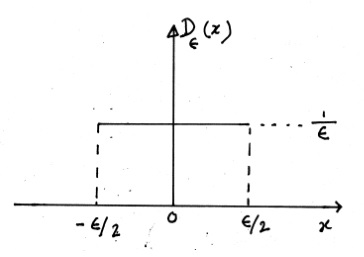
\includegraphics[width=80mm]{rep1.jpg}
\caption{Plot of the function defined in Eq. (\ref{eq:rep1})}
\end{figure}

\noindent
The integral of the function with respect to $x$ is unity, i.e.,
\be
\int_{-\infty}^{\infty} D_{\epsilon}(x) dx =1.
\ee
Now, imagine making $\epsilon$ smaller. As we decrease $\epsilon$, the function gets narrower and taller, but the integral
of the function (i.e., the area under the graph of the function) remains constant at the value 1. In the limit
$\epsilon \rightarrow 0$, the function $D_{\epsilon}(x)$ collapses to a single point, namely $x=0$, and gets infinitely tall. So,
$\lim_{\epsilon\rightarrow 0}D_{\epsilon}(x)$ is not a function at all and the procedure of taking the limit
$\epsilon \rightarrow 0$ is not justified.

\paragraph{}
However, we can make the limiting procedure meaningful if we multiply $D_{\epsilon}(x)$ by some well-defined function
$f(x)$, integrate over $x$ and then take the limit $\epsilon \rightarrow 0$. Consider the integral
\[ \int_{-\infty}^{\infty} D_{\epsilon}(x)f(x)dx \]
where $f(x)$ is a well-defined function. If $\epsilon$ is sufficiently small, the variation of $f(x)$ over the effective
integration interval $[-\epsilon/2,\epsilon/2]$ is negligible and $f(x)$ remains practically equal to $f(0)$. Therefore,
\be
\int_{-\infty}^{\infty} D_{\epsilon}(x)f(x) dx \approx f(0) \int_{-\infty}^{\infty} D_{\epsilon}(x)dx = f(0).
\ee
The smaller the value of $\epsilon$, the better the approximation. In the limit $\epsilon \rightarrow 0$, the above equation is exact:
\be
\lim_{\epsilon \rightarrow 0}\int_{-\infty}^{\infty}D_{\epsilon}(x)f(x)dx = f(0).
\ee
Now, we define the Dirac Delta Function $\delta(x)$ as
\be
\int_{-\infty}^{\infty}\delta(x) f(x)dx \stackrel{{\rm def}}= \lim_{\epsilon \rightarrow 0}\int_{-\infty}^{\infty}D_{\epsilon}(x)f(x)dx = f(0)
\ee
This equation is valid for any function $f(x)$  defined at the origin. More generally, $\delta(x-x_0)$ is defined as
\be
\int_{-\infty}^{\infty} \delta(x-x_0)f(x)dx = f(x_0).
\ee

\paragraph{}
Actually, the integral notation
\[ \int_{-\infty}^{\infty}\delta(x)f(x)dx\]
is not justified because $\delta(x)$ is not really a function. Physically, there is no problem since it becomes impossible to distinguish
between $D_{\epsilon}(x)$ and $\delta(x)$ as soon as $\epsilon$ becomes negligible compared to all distances involved in a physical problem.
Whenever a mathematical difficulty might arise, all we need to do is to assume that $\delta(x)$ is actually $D_{\epsilon}(x)$ with
$\epsilon$ extremely small but not strictly zero.

\paragraph{}
Formally, we can express $\delta(x)$ as a limit of a sequence of proper functions:
\be
\lim_{\epsilon \rightarrow 0}D_{\epsilon}(x) \equiv \delta(x).
\ee
Here $D_{\epsilon}(x)$, which is a proper function of $x$, is called the representation of the delta function. The representation we have discussed so far is the ``square function" given in Eq. (\ref{eq:rep1}). The representation is not unique. There are other functions which 
approach the delta function when appropriate limits are taken.

\subsubsection{\underline{Gaussian Representation}}
Consider the function
\be
D_{\epsilon}(x) =\frac{1}{\epsilon \sqrt{\pi}}e^{-x^2/\epsilon^2} \;\; (\epsilon>0).
\label{eq:rep2}
\ee
For each value of the parameter $\epsilon$, this function satisfies
\be
\int_{-\infty}^{\infty}D_{\epsilon}(x) dx =1.
\ee
This  is the normalized Gaussian function whose plot is shown in the figure below.
\begin{figure}[ht]
\centering
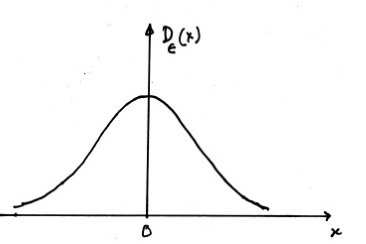
\includegraphics[width=80 mm]{rep2.jpg}
\caption{Plot of the Gaussian function defined in Eq. (\ref{eq:rep2})}
\end{figure}

\noindent
The Gaussian function has a peak at the origin. The peak has a height $1/\epsilon\sqrt{\pi}$ and a width of order $\epsilon$
(exactly how the width is defined doesn't matter). So if $\epsilon$ is allowed to be very small, the peak becomes very tall and very 
narrow. Outside the peak the function becomes extremely small. Thus we have
\be
\delta(x) = \lim_{\epsilon \rightarrow 0} \frac{1}{\epsilon \sqrt{\pi}} e^{-x^2/\epsilon^2}.
\ee

\vspace{10 mm}
\noindent
{\bf Mathematical Notes:} \newline
\noindent
We have the integral
\[ \int_{-\infty}^{\infty}e^{-x^2}dx = \sqrt{\pi}. \]
Now let us consider the following integral
\[ I= \int_{-\infty}^{\infty}e^{-b^2x^2+ a x}dx.\]
First, write
\[ b^2x^2+ax = \left(bx+\frac{a}{2b}\right)^2-\frac{a^2}{4b^2} .\]
Therefore,
\begin{eqnarray*}
I & =& e^{a^2/4b^2}\int_{-\infty}^{\infty}e^{-(bx+a/2b)^2}dx \\
& = & e^{a^2/4b^2}(1/b)\int_{-\infty}^{\infty}e^{-z^2}dz \quad (z=bx+\frac{a}{2b}) \\
& = & e^{a^2/4b^2}\frac{\sqrt{\pi}}{b}.
\end{eqnarray*}

\subsubsection{\underline{Damped Sinusoidal Representation of the Delta Function}}
Consider another function
\be
D_{\epsilon}(x) = \frac{1}{\pi}\, \frac{\sin (x/\epsilon)}{x}\quad (\epsilon > 0).
\label{eq:rep3}
\ee
A plot of the function is shown below.
\begin{figure}[ht]
\centering
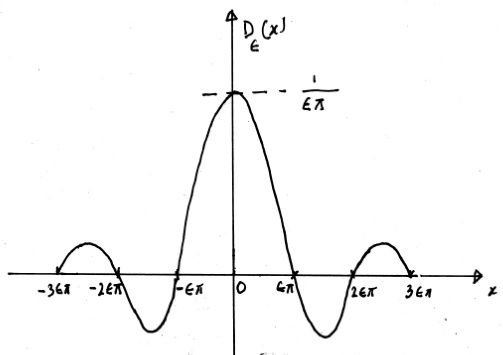
\includegraphics[width=100 mm]{rep3.jpg}
\caption{Plot of the function defined in Eq. (\ref{eq:rep3})}
\end{figure}
The function $D_{\epsilon}(x)$ has the value $1/\epsilon\sqrt{\pi}$ at $x=0$ and it oscillates with decreasing amplitude
as $|x|$ increases. The width of the central maximum is of the order of $\epsilon$ and the period of oscillations with respect to
$x$ is $2\pi \epsilon$.



\noindent
For any value of $\epsilon$ we have
\be
\int_{-\infty}^{\infty} D_{\epsilon}(x)dx = 1.
\ee


\paragraph{}
Thus, the limit of the function as $\epsilon \rightarrow 0$ has all the properties of the delta function: it becomes infinitely large
at $x=0$, and infinitely rapid oscillations as $|x|$ increases means that the entire contribution to an integral containing this
function comes from an infinitesimal neighborhood of $x=0$. We can therefore write
\be
\delta(x) = \lim_{\epsilon \rightarrow 0} \frac{1}{\pi}\, \frac{\sin(x/\epsilon)}{x}
\ee

\vspace{10 mm}
\subsubsection{\underline{Other representation of the Delta Function}}
We can also show that
\begin{eqnarray}
\delta(x) &=& \lim_{\epsilon \rightarrow 0} \frac{1}{2\epsilon}\, e^{-|x|/\epsilon} \\
\delta(x) &=& \lim_{\epsilon \rightarrow 0} \frac{1}{\pi}\, \frac{\epsilon}{x^2+\epsilon^2} \\
\delta(x) &=& \lim_{\epsilon \rightarrow 0} \frac{\epsilon}{\pi}\, \frac{\sin^2(x/\epsilon)}{x^2}.
\end{eqnarray}



\section{Properties of the Delta Function}
It is important to note that, because of its singular character, the $\delta$-function cannot be the end result of a calculation,
and has meaning only so long as a subsequent integral over its argument is carried out. With this understanding we can write
down some relations between delta functions:
\begin{enumerate}
\item
The delta function is an even function, i.e.,
\be
\delta(-x)=\delta(x).
\ee

\item
\be
x\delta(x)=0.
\ee

\item
\be
\delta(ax) = \frac{1}{|a|} \delta(x).
\ee
{\bf Proof:}\newline
Consider the integral
\[
I=\int_{-\infty}^{\infty}\delta(ax)f(x)dx. 
\]
Since the delta function is an even function it doesn't matter if we replace $a$ by $|a|$ in the argument. Thus
\[ I= \int_{-\infty}^{\infty} \delta(|a|x)f(x) dx \, . \]
Making the change of variable
\[ y=|a|x \]
we have
\[ I= \frac{1}{|a|} \int_{-\infty}^{\infty} \delta(y)f(y/|a|) dy= \frac{1}{|a|} f(0) \, , \]
or,
\[ \int_{-\infty}^{\infty} \delta(ax)f(x) dx  = \frac{1}{|a|} \int_{-\infty}^{\infty} \delta(x)f(x) dx \, , \]
i.e.,
\begin{equation*}
\boxed{
\delta(ax)=\frac{1}{|a|}\delta(x)
}
\end{equation*}

\item
More generally, we have
\be
\delta(\phi(x)) = \sum_i \frac{\delta(x-x_i)}{\left|\frac{\partial\phi}{\partial x}\right|_{x_i}}
\ee
where the sum runs over the $x_i$'s which are the simple roots of $\phi(x)$.

\noindent
{\bf Proof:}\newline
Let $x_1, x_2, \cdots , x_N$ be the simple roots of $\phi(x)$ (figure below):
\begin{figure}[ht]
\centering
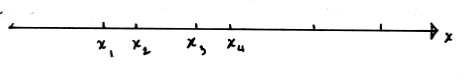
\includegraphics[width=80 mm]{roots.jpg}
\caption{Simple roots of $\phi(x)$.}
\end{figure}

\noindent
In the neighborhood of any of the simple roots $x_i$, we can write
\[ \phi(x) = (x-x_i)\psi(x) \]
where $\psi(x_i) \neq 0$. We have
\[ \psi(x_i) = \left. \frac{\partial \phi(x)}{\partial x}\right|_{x=x_i}. \]

Now, consider the integral
\begin{eqnarray*}
\int_{-\infty}^{\infty} \delta(\phi(x))f(x)dx &=& \sum_{i=1}^N\int_{x_i-\epsilon}^{x_i+\epsilon}
\delta\left[(x-x_i)\psi(x_i)\right]f(x)dx \\
& = & \sum_{i=1}^N  \frac{1}{|\psi(x_i)|}  \int_{x_i-\epsilon}^{x_i+\epsilon} \delta(x-x_i)f(x)dx \\
& = & \sum_{i=1}^N\frac{1}{|\frac{\partial \phi}{\partial x}|_{x=x_i}}  \int_{-\infty}^{\infty} \delta(x-x_i)f(x)dx \\
& = & \sum_{i=1}^N\frac{1}{|\frac{\partial \phi}{\partial x}|_{x=x_i}}  f(x_i) 
\end{eqnarray*}
The above result is obtained if we write
\be
\delta(\phi(x)) = \sum_{i=1}^N \frac{\delta(x-x_i)}{~~\left| \frac{\partial \phi}{\partial x} \right|_{x=x_i} }. \quad {\rm Proved.}
\ee

\item
A frequently used example of the above result is
\be
\delta(x^2-a^2) = \frac{1}{2a}\delta(x-a) + \frac{1}{2a}\delta(x+a), \;\;\; (a>0).
\ee
Here
\[ \phi(x) = x^2-a^2 = (x-a)(x+a). \]
The two simple roots of $\phi(x)$ are at $x=a$ and $x=-a$. Now
\[ \left| \frac{\partial \phi}{\partial x}\right|_{x=a} = |2x|_{x=a} = 2a \]
and
\[ \left| \frac{\partial \phi}{\partial x}\right|_{x=-a} = |2x|_{x=-a} = 2a .\]
Therefore, the above result follows.

\item
\[ f(x)\delta(x-a) = f(a)\delta(x-a).\]

\item
\[ \int \delta(x-y)\delta(y-a) dy = \delta(x-a). \]

\end{enumerate}

\noindent
{\bf Note 1:}\newline
We have the identity
\[ x\delta(x) = 0. \]
The converse is also true and it can be shown that the equation
\[ xu(x)=0 \]
has the general solution
\[ u(x) = c \delta(x).\]

\vspace{10 mm}
\noindent {\bf Note 2:}\newline
We will now prove an identity which is particularly useful in quantum mechanics:
\be
\lim_{\epsilon \rightarrow 0^+} \int_{-\infty}^{\infty} \frac{1}{x \pm  i\epsilon}\, f(x)dx =
\mathcal{P} \int_{-\infty}^{\infty}\frac{dx}{x} f(x)  \mp i\pi f(0),
\ee
or, in short 
\be
\lim_{\epsilon \rightarrow 0^+} \frac{1}{x\pm i\epsilon} = \mathcal{P} \left( \frac{1}{x} \right) \mp i\pi \delta(x),
\ee
where it is understood that the second of these two equations have meaning only within an integral. The symbol $\mathcal{P}$
means the the principal part of an integral where the integrand has a simple pole. The principal part is defined as
\be
\mathcal{P} \int_{-A}^{B} \frac{dx}{x} f(x) = \lim_{\eta \rightarrow 0^+}\left[ \int_{-A}^{-\eta} + \int_{\eta}^B\right]
\frac{dx}{x} f(x).
\ee

\noindent
{\bf Proof:}\newline
We can write
\be
\frac{1}{x\pm i\epsilon} = \frac{x\mp i\epsilon}{x^2+\epsilon^2}= \frac{x}{x^2+\epsilon^2} \mp \frac{i\epsilon}{x^2+a^2}.
\label{eq:pv1}
\ee
Now, we have
\[ \lim_{\epsilon \rightarrow 0^+} \frac{1}{\pi}\, \frac{\epsilon}{x^2+ \epsilon^2} = \delta(x). \]
Therefore,
\be
\lim_{\epsilon \rightarrow 0^+} (\mp) i \frac{\epsilon}{x^2+a^2} = \mp i\pi \delta(x).
\ee
Next, consider the first term on the right and side of Eq. (\ref{eq:pv1}). We multiply this term by a function $f(x)$ which is regular 
at the origin and then integrate over $x$. We get

\begin{multline}
\lim_{\epsilon \rightarrow 0^+} \int_{-\infty}^{\infty}\frac{xf(x)}{x^2+a^2} dx \\
= \lim_{\epsilon \rightarrow 0^+} \left[ \lim_{\eta \rightarrow 0^+} \int_{-\infty}^{-\eta}\frac{xf(x)}{x^2+a^2} dx 
+ \lim_{\eta \rightarrow 0^+} \int_{-\eta}^{\eta}\frac{xf(x)}{x^2+a^2} dx 
+ \lim_{\eta \rightarrow 0^+} \int_{\eta}^{\infty}\frac{xf(x)}{x^2+a^2} dx \right]
\label{eq:pv2}
\end{multline}
Note that we take the limit over $\eta$ first and the we take the limit over $\eta$. Now consider the second integral of the above equation.
\[
\lim_{\eta \rightarrow 0^+} \int_{-\eta}^{\eta}\frac{xf(x)}{x^2+a^2} dx= f(0) \lim_{~\eta \rightarrow 0^+}
\frac{1}{2} \left[ \ln (x^2+ \epsilon^2) \right]_{x=-\eta}^{x=\eta} = 0.
\]
If we now reverse the order of the evaluation of limits in Eq. (\ref{eq:pv2}), the $\epsilon \rightarrow 0^+$ limit
causes no difficulties in the other two integrals. We thus have
\begin{eqnarray*}
\lim_{\epsilon \rightarrow 0^+} \int_{-\infty}^{\infty}\frac{xdx}{x^2+a^2}f(x) &=& \lim_{\eta \rightarrow 0^+}
\lim_{\epsilon \rightarrow 0^+}\left[ \int_{-\infty}^{-\eta} + \int_{\eta}^{\infty}\right] \frac{xdx}{x^2+a^2}f(x) \\
&=& \lim_{\eta \rightarrow 0^+} \left[ \int_{-\infty}^{-\eta} + \int_{\eta}^{\infty}\right] \frac{dx}{x}f(x)\\
&=& \mathcal{P}  \int_{-\infty}^{\infty} \frac{1}{x} f(x)dx
\end{eqnarray*}
This establishes the identity.


\section{Derivative of the Delta Function}
One may define the derivative $\delta^{\prime}(x)$ of the delta function. When $\epsilon$ is small, the derivative of 
$D_{\epsilon}(x)$ has two peaks close to the origin, one peak being positive and the other negative as shown in the figure
below.
\begin{figure}[ht]
\centering
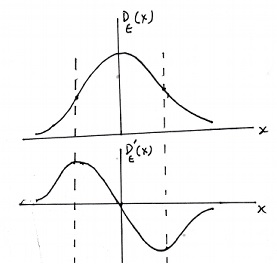
\includegraphics[width=90 mm]{derivative.jpg}
\caption{Plot of $D_{\epsilon}(x)$ and $D^{\prime}_{\epsilon}(x)$.}
\end{figure}


\noindent
As $\epsilon \rightarrow 0$, each of the peaks become very narrow and very tall, and each of the two peaks approach very close to the
origin.  Now, an integration by parts gives
\be
\int_{-\infty}^{\infty} D_{\epsilon}^{\prime}(x)f(x) dx = \left[ D_{\epsilon}(x)f(x)\right]_{-\infty}^{\infty}
- \int_{-\infty}^{\infty} D_{\epsilon}(x) f^{\prime}(x) dx\, . 
\ee
Because $D_{\epsilon}(x)$ tends to zero as $x \rightarrow \pm \infty$, the first term on the right hand side vanishes unless
$f(x)$ explodes violently at infinity. So by letting $\epsilon \rightarrow 0$, we arrive at the definition of
$\delta^{\prime}(x)$:
\be
\boxed{
\int_{-\infty}^{\infty} \delta^{\prime}(x) f(x) dx = - \int_{-\infty}^{\infty}\delta(x)f^{\prime}(x) dx = -f^{\prime}(0).
}
\label{eq:deltaprime}
\ee
From this we immediately get 
\be
\boxed{
x\delta^{\prime}(x) =-\delta(x).
}
\ee
Conversely, it can be shown that the general solution of the equation
\[ xu(x) = \delta(x) \]
can be written as
\[ u(x) =-\delta^{\prime}(x) + c \delta(x) \]
where the second term arises from the homogeneous equation
\[ x\delta(x) = 0. \]
From the definition (\ref{eq:deltaprime}) it also follows that
\be
\boxed{
\delta^{\prime}(-x) = - \delta^{\prime}(x).
}
\ee
The $n^{th}$ order derivative of $\delta(x)$ can be defined in the same way. We find
\be
\int_{-\infty}^{\infty} \delta^{(n)}(x) f(x) dx = (-1)^n f^{(n)}(0).
\ee
We can also prove the following properties of the derivatives of the delta function:
\begin{eqnarray*}
\delta^{(m)}(x)& = &(-1)^m \delta^{(m)}(-x)  \\
x^{m+1}\delta^{(m)}(x)& = & 0  \\
x \delta^{(m)}(x)& = &-(m-1) \delta^{(m-1)}(x).
\end{eqnarray*}


\section{Integration of the Delta Function}
Consider the indefinite integral
\be
\theta_{\epsilon}(x) = \int_{-\infty}^x D_{\epsilon}(y)dy .
\label{eq:theta}
\ee
A graph of $\theta_{\epsilon}(x)$ versus $x$ is shown below.
\begin{figure}[ht]
\centering
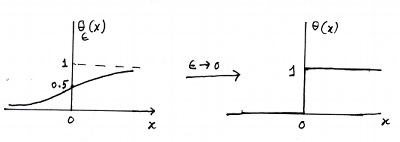
\includegraphics[width=\linewidth]{theta.jpg}
\caption{The $\theta$-function as an integral of the delta function}
\end{figure}


\noindent
As $\epsilon \rightarrow 0$, the step in the function $\theta_{\epsilon}(x)$ gets progressively steeper, until, finally, the function changes abruptly from 0 to 1 at $x=0$. Therefore, taking the limit $\epsilon \rightarrow 0$ in Eq. (\ref{eq:theta})
we have
\be
\theta(x) = \int_{-\infty}^x\delta(y)dy
\label{eq:theta2}
\ee
where
\be
\theta(x) = \left\{ \begin{array}{cl}
                     1 & {\rm for}\; x>0 \\
										0 & {\rm for}\; x<0.
										\end{array} \right.
\ee										
If we differentiate Eq. (\ref{eq:theta2}) with respect to $x$, we get
\be
\frac{d\theta(x)}{dx} = \delta(x).
\ee


\section{Three dimensional delta function}
The three-dimensional delta function $\delta(\vec{r}\,)$ is defined as
\be
\delta(\vec{r}\,) \stackrel{{\rm def}} \equiv \delta(x) \delta(y) \delta(z).
\ee
In other words, $\delta(\vec{r}\,)$ is zero if any of the coordinates $x$, $y$ and $z$ is {\underline{not}} equal to 
zero and $\delta(\vec{r}\,)$ tends to infinity at the origin, i.e., when $x=0$, $y=0$ and $z=0$, such that
\be
\int_{{\rm volume}}\delta(\vec{r}\,)d^3r = 1
\ee
if the volume of integration contains the origin. We also have
 \be
\int \delta(\vec{r}\,)f(\vec{r}\,)d^3r = f(0)
\ee
where again the volume of integration contains the origin. 

\vspace{10 mm}
\noindent
{\bf Note:}
\begin{itemize}
\item
$\delta(\vec{r} - \vec{r}^{\;\prime}\, ) = \delta(x-x^{\prime})\delta(y-y^{\prime})\delta(z-z^{\prime})$
\item $ \int_{V} \delta(\vec{r} - \vec{r}^{\;\prime}\, )d^3r =1 $
\newline
where the volume of integration includes the point $\vec{r}^{\;\prime}$. Otherwise, the integral is zero.
\item $ \int_{V} \delta(\vec{r} - \vec{r}^{\;\prime}\, ) f(\vec{r}\,)d^3r = f(\vec{r}^{\; \prime})$ \newline
if $V$ includes the point $\vec{r}^{\;\prime}$.

\end{itemize}



\subsubsection{A useful formula}
Consider the integral
\begin{eqnarray*}
\int_{-\infty}^{\infty}e^{ikx} dx &=& \lim_{L\rightarrow \infty} \int_{-L}^{L} e^{ikx}dx \\
&=& \lim_{L\rightarrow \infty} \frac{1}{ik}\, \left(e^{ikL}-e^{-ikL} \right) \\
&=& \lim_{L\rightarrow \infty} \, \frac{2}{k} \left( \frac{ e^{ikL}-e^{-ikL}}{2i} \right) \\
&=& \lim_{L\rightarrow \infty}\, \frac{2}{k}\sin kL \\
&=& 2\pi \lim_{L\rightarrow \infty}\, \frac{\sin kL}{\pi k}\\
&=& 2\pi \delta(k),
\end{eqnarray*}
where we have used
\be
\lim_{\epsilon \rightarrow 0} \frac{ \sin (x/\epsilon)}{\pi x} = \delta(x).
\ee
Thus, we have the very important formula
\be
\boxed{
\int_{-\infty}^{\infty}e^{ikx}dx = 2\pi \delta(k)
}
\label{eq:ft3}
\ee
In Eq. (\ref{eq:ft3}) if we integrate with respect to $k$, we would have $\delta(x)$ on the right hand side,
\be
\boxed{
\int_{-\infty}^{\infty}e^{ikx}dk = 2\pi \delta(x)
}
\label{eq:ft4}
\ee
Also note that in Eq. (\ref{eq:ft3}) we integrate over the full domain of $x$ from $-\infty$ to $\infty$. Making a change of variable $x\rightarrow -x$ does not change the value of the integral. Hence we also have
\be
\boxed{
\int_{-\infty}^{\infty}e^{-ikx}dx = 2\pi \delta(k)
}
\label{eq:ft5}
\ee
Similarly, in Eq. (\ref{eq:ft4}), making the change of variable $k \rightarrow -k$, doesn't change the value of the integral. So we could also write
\be
\boxed{
\int_{-\infty}^{\infty}e^{-ikx}dk = 2\pi \delta(x)
}
\label{eq:ft6}
\ee
Thus, in summary
\be
\int_{-\infty}^{\infty}e^{\pm ikx}dx = 2\pi \delta(k),
\ee
and
\be
\int_{-\infty}^{\infty}e^{\pm ikx}dk = 2\pi \delta(x),
\ee
In three dimensions we have
\be
\int_{{\rm all\; space}}e^{\pm i\vec{k}.\vec{r}}d^3r = (2\pi)^3 \delta(\vec{k}\,).
\ee
\be
\int_{{\rm all\; space}}e^{\pm i(\vec{k}-\vec{k}^{\;\prime}).\vec{r}}d^3r = (2\pi)^3 \delta(\vec{k}-\vec{k}^{\;\prime}\,).
\ee
\be
\int_{{\rm all\; space}}e^{\pm i \vec{k}.(\vec{r}-\vec{r}^{\;\prime})}d^3k = (2\pi)^3 \delta(\vec{r}-\vec{r}^{\;\prime}\,).\ee


\section{Fourier transform}

We can always express a function $f(x)$ in the form
\be
f(x) = \int_{-\infty}^{\infty}e^{ikx}\tilde{f}(k)dk
\label{eq:ft10}
\ee
where $\tilde{f}(k)$ is a function of $k$, called the Fourier transform of $f(x)$. From Eq. (\ref{eq:ft10}) we can write
\begin{eqnarray*}
\int_{-\infty}^{\infty}e^{-ik^{\prime}x}f(x)dx &=& \int_{-\infty}^{\infty}\int_{-\infty}^{\infty}e^{i(k-k^{\prime}\,)x}
\tilde{f}(k)dkdx \\
&=& 2\pi \int_{-\infty}^{\infty}\delta(k-k^{\prime}\,)\tilde{f}(k)dk \\
&=& 2\pi \tilde{f}(k^{\prime}\,)
\end{eqnarray*}
Thus, 
\be
\tilde{f}(k) = \frac{1}{2\pi}\int_{\infty}^{\infty}e^{-ikx}f(x)dx.
\label{eq:ft11}
\ee
The functions $f(x)$ and $\tilde{f}(k)$ are Fourier transform of each other. We can write Eqs. (\ref{eq:ft10}) 
and (\ref{eq:ft11}) in a more symmetrical fashion as follows
\begin{eqnarray}
f(x)& = &\frac{1}{\sqrt{2\pi}} \int_{-\infty}^{\infty}e^{ikx}\tilde{f}(k)dk \\
\tilde{f}(k) &=& \frac{1}{\sqrt{2\pi}}\int_{\infty}^{\infty}e^{-ikx}f(x)dx.
\end{eqnarray}

\paragraph{}
In three dimensions we can write
\be
f(\vec{r}\,) = \frac{1}{(2\pi)^{3/2}} \int e^{i\vec{k}.\vec{r}} \tilde{f}(\vec{k}\,)d^3k.
\ee
Multiplying this equation by $e^{-i\vec{k}^{\; \prime}.\vec{r}}$ and integrating over $\vec{r}$, we have
\begin{eqnarray*}
\int_{{\rm all\; space}} e^{-i\vec{k}^{\; \prime}.\vec{r}} f(\vec{r}\,)d^3r
&=& \frac{1}{(2\pi)^{3/2}} \int d^3r\int d^3k\, e^{i(\vec{k}-\vec{k}^{\; \prime}).\vec{r}}\tilde{f}(\vec{k}\,) \\
&=& \frac{1}{(2\pi)^{3/2}} \int d^3k\, (2\pi)^{3} \delta(\vec{k}-\vec{k}^{\; \prime})\tilde{f}(\vec{k}\,) \\
&=& (2\pi)^{3/2} \tilde{f}(\vec{k}^{\; \prime}\,)
\end{eqnarray*}
Therefore,
\be
\tilde{f}(\vec{k}\,) = \frac{1}{(2\pi)^{3/2}}\int e^{-i\vec{k}.\vec{r}} f(\vec{r}\,)d^3r.
\ee


\noindent
In summary, 

\begin{eqnarray}
f(\vec{r}\,)& =& \frac{1}{(2\pi)^{3/2}} \int e^{i\vec{k}.\vec{r}} \tilde{f}(\vec{k}\,)d^3k, \\
\tilde{f}(\vec{k}\,)& =& \frac{1}{(2\pi)^{3/2}}\int e^{-i\vec{k}.\vec{r}} f(\vec{r}\,)d^3r.
\end{eqnarray}


\newpage

\subsection{Parseval Identity}
We will now prove the important identity
\be
\int \left|f(\vec{r}\,)\right|^2d^3r = \int \left| \tilde{f}(\vec{k}\,)\right|^2d^3k.
\ee

\vspace{5 mm}
{\bf \underline{Proof}:}
\begin{multline}
\int \left|f(\vec{r}\,)\right|^2d^3r = \int f(\vec{r}\,) f^*(\vec{r}\,)d^3r \\
=\int d^3r \, \frac{1}{(2\pi)^{3/2}} \int e^{i\vec{k}.\vec{r}} \tilde{f}(\vec{k}\,)d^3k \,
\frac{1}{(2\pi)^{3/2}}   \int e^{-i\vec{k}^{\; \prime}.\vec{r}} \tilde{f}^*(\vec{k}^{\; \prime}\,)d^3k^{\prime}~~~~\\
=\frac{1}{(2\pi)^3}\int d^3k d^3k' \tilde{f}(\vec{k}\,) \tilde{f}^*(\vec{k}^{\; \prime}\,)
\underbrace{ \int d^3r\, e^{i(\vec{k}-\vec{k}^{\; \prime}\,).\vec{r}} }_{(2\pi)^3 \delta(\vec{k}-\vec{k}^{\; \prime}\,) }
\qquad \qquad \qquad ~~~\\
= \int d^3k d^3k' \tilde{f}(\vec{k}\,) \tilde{f}^*(\vec{k}^{\; \prime}\,)\delta(\vec{k}-\vec{k}^{\; \prime}\,) \qquad
\qquad \qquad \qquad \qquad ~~~~~~\\
= \int d^3k  \tilde{f}(\vec{k}\,) \tilde{f}^*(\vec{k}\,) \qquad \qquad \qquad \qquad \qquad\qquad\qquad\qquad
~~~~~ \\
= \int d^3k \left | \tilde{f}(\vec{k}\,) \right|^2. \qquad \qquad \qquad \qquad \qquad \qquad \qquad \qquad \qquad ~~
\end{multline}

The proof is now complete.


					







\begin{titlepage}
\begin{center}
        
\vspace*{5cm}
        
\Huge
\textbf{DIRAC DELTA FUNCTION \\ FOR \\ STUDENTS IN A HURRY}

\vspace*{1cm}

\large
\textbf{\textit{by}}

\vspace*{1cm}
\Large
\textbf{Prof. Dr. Khorshed Ahmed Kabir}

\end{center}

\end{titlepage}



\section*{Dirac Delta Function}
Consider the function $D_\epsilon (x)$ given by 
\begin{align*}
D_\epsilon (x) & = \frac{1}{\epsilon} \ \ ;\ for -\frac{\epsilon}{2} \leq x \leq \frac{\epsilon}{2} \\
& = 0 \ \ \ ;\ for \ |x| > \frac{\epsilon}{2}
\end{align*}
where $\epsilon$ is a positive parameter. The plot of the function is shown below.

\vspace{0.2cm}
\begin{center}
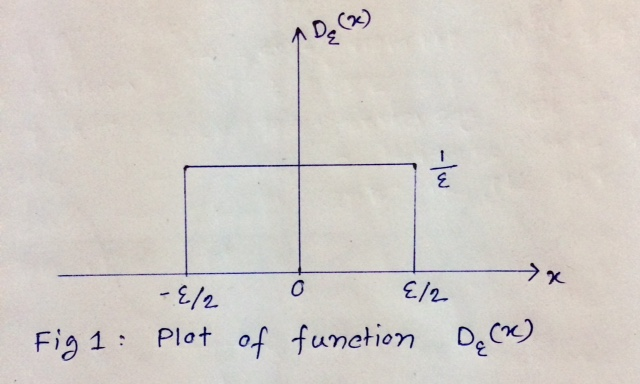
\includegraphics[width=0.5\textwidth]{DiracDeltaFig1.jpg}
\end{center}

The integral of the function with respect to x is 1, i.e,
\begin{equation}
\int_{-\infty}^\infty D_\epsilon (x) dx = 1 
\end{equation}

Now imagine making $\epsilon$ smaller. As we decrease $\epsilon$, the function gets narrower and taller, but the integral of the function i.e, the area under the graph remain constant at the value 1. In the limit $\epsilon \to 0$, the function $D_{\epsilon} (x)$ collapses to a single point $x=0$ and gets infinitely tall. So, $\lim_{\epsilon \to 0} D_\epsilon (x)$ is not a function at all and the procedure of taking the limit $\epsilon \to 0$ is not justified.\\

However, we can make the limiting procedure meaningful if multiply $D_\epsilon (x)$ by some well defined function $f(x)$, integrate over x and then take the limit $\epsilon \to 0$. Consider, the integral $$\int_{-\infty}^\infty D_\epsilon (x) f(x) dx $$ where $f(x)$ is a well defined function. If $\epsilon$ is significantly small, the variation of $f(x)$ over the effective integration interval $[-\frac{\epsilon}{2},\frac{\epsilon}{2}]$ is negligible and $f(x)$ remain practically equal to f(0). Therefore,
\begin{equation}
\int_{-\infty}^{\infty} D_\epsilon (x) f(x) dx \ \simeq f(0) \int_{-\infty}^{\infty} D_\epsilon (x) dx = f(0)
\end{equation}
The smaller the value of $\epsilon$, the better the approximation. in the limit $\epsilon \to 0$, the above equation is exactly
\begin{equation}
\lim_{\epsilon \to 0} \int_{-\infty}^{\infty} D_\epsilon (x) f(x) dx = f(0)
\end{equation} 
Now, we define the delta function by the relation
\begin{equation}
\int_{-\infty}^\infty \delta (x) f(x) dx = \lim_{\epsilon \to 0} \int_{-\infty}^{\infty} D_\epsilon (x) f(x) dx = f(0)
\end{equation}
This equation is valid for any function defined at the origin. More generally, $\delta (x-x_0)$ is defined as
\begin{equation}
\int_{-\infty}^\infty \delta (x-x_0) f(x) dx = f(x_0)
\end{equation}
Actually, the integral notation $\int_{-\infty}^\infty \delta (x) f(x) dx $ is not justified because $\delta(x)$ is not really a function. Physically, there is no problem since it becomes impossible to distinguish between $D_\epsilon (x)$ and $\delta (x)$ as soon as $\epsilon$ becomes negligible compared to all the distances involved in a physical problem. Whenever a mathematical difficulty arise, all we need to do is to assume that $\delta (x)$ is actually $D_\epsilon (x)$ with $\epsilon$ extemely small but not strictly zero.\\

Formally, we can express $\delta(x)$ as a sequence of proper functions $$\lim_{\epsilon \to 0} D_\epsilon (x) \equiv \delta(x) $$ Here, $D_\epsilon (x)$, which is a proper function of x is called the representation of the delta function. One representation is the 'Square Function' given at the beginning. The representation is not unique. There are other functions which approach the delta function when appropriate limits are taken.

\section*{Other Representation Of The Delta Function}
\subsection*{A}
Consider the function 
\begin{equation}
D_\epsilon (x) = \frac{1}{\epsilon \sqrt{\pi}} e^{-x^2/\epsilon^2} \ \ \ with\ \ \epsilon > 0
\end{equation}
For each value of the parameter $\epsilon$, this function satisfies $$\int_{-\infty}^\infty D_\epsilon (x)dx =1$$ 

\vspace{0.2cm}
\begin{center}
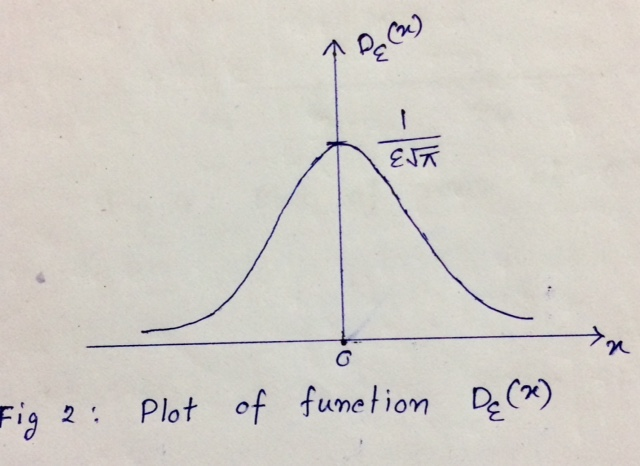
\includegraphics[width=0.5\textwidth]{DiracDeltaFig2.jpg}
\end{center}
When plotted against x, the function has a peak at the origin. The peak has a height $\frac{1}{\epsilon \sqrt{\pi}}$ and a width of order $\epsilon$ (exactly how the width is defined doesn't matter). So, if $\epsilon$ is allowed to become very small, the peak becomes very tall and very narrow. Outside the peak, the function becomes extremely small. Thus we have 
\begin{equation}
\delta (x) = \lim_{\epsilon \to 0} \frac{1}{\epsilon \sqrt{\pi}} e^{-x^2/\epsilon^2}
\end{equation}
\\\\
Note: $$\int_{-\infty}^{\infty} e^{-x^2}dx = \sqrt{\pi}$$
Let, 
\begin{align*}
I &= \int_{-\infty}^{\infty} e^{-(b^2 x^2 + ax)} dx \\
&=e^{a^2/4b^2} \int_{-\infty}^{\infty} e^{-(bx + a/2b)^2} dx \\
&= e^{a^2/4b^2} \frac{1}{b} \int_{-\infty}^{\infty} e^{-z^2} dz \\
&= e^{a^2/4b^2} \frac{\sqrt{\pi}}{b}
\end{align*}
By using $$ b^2 x^2 + ax = (bx + \frac{a}{2b})^2 - \frac{a^2}{4b^2}$$ and by letting $$ z= bx+\frac{a}{2b}$$

\subsection*{B}
Consider another function
\begin{equation}
D_{\epsilon} (x) = \frac{1}{\pi} \frac{\sin (x/\epsilon)}{x} \ \ \ with\ \epsilon>0
\end{equation}

\vspace{0.2cm}
\begin{center}
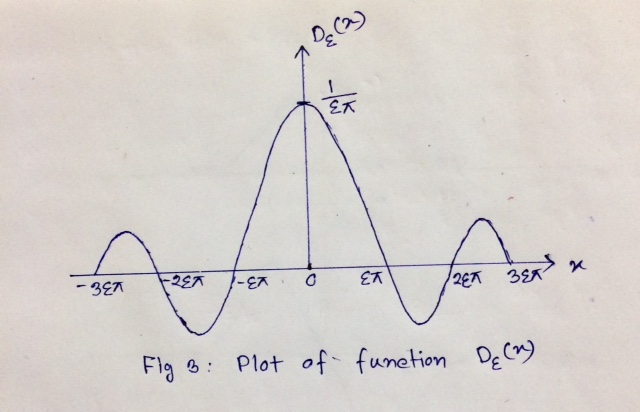
\includegraphics[width=0.6\textwidth]{DiracDeltaFig3.jpg}
\end{center}

For any value of the parameter $\epsilon$ we have 
\begin{equation}
\int_{-\infty}^{\infty} D_\epsilon (x) dx = 1
\end{equation}
A plot of the function $D_{\epsilon} (x)$ shows that it has the value $\frac{1}{\epsilon \pi}$ at x=0 and it oscillates with decreasing amplitude as $|x|$ increases. The width of the central maxima is of the order of $\epsilon$ and the period of oscillation with respect tox is $2\pi \epsilon$.

Thus the limit of the function as $\epsilon \to 0$ has all the properties of the delta function: it becomes infintely large at x=0, it has unit integral, and infinitely rapid oscillations as $|x|$ increases means that the entire contribution to an integral containing this function comes from an infinitesimal neighbourhood of x=0. We can therefore write 
\begin{equation}
\delta (x) = \lim_{\epsilon \to 0} \frac{1}{\pi} \frac{\sin (x/\epsilon)}{x}
\end{equation}

\subsection*{C}
We can also show that $$\delta (x) = \lim_{\epsilon \to 0} \frac{1}{2\epsilon} e^{-|x|/\epsilon}$$  $$\delta (x) = \lim_{\epsilon \to 0} \frac{1}{\pi} \frac{\epsilon}{x^2 + \epsilon^2}$$  $$\delta (x) = \lim_{\epsilon \to 0} \frac{\epsilon}{\pi} \frac{\sin^2 (x/\epsilon)}{x^2}$$


\section*{Properties Of The Delta Function}
It is important  to note that, because of its singular character, the delta function can not be the end result of a calculation and has meaning only so long as a subsequent integral over its argument is carried out. With this understanding we can write down some relations between delta functions.

\textbf{1.} The delta function is an even function: $$
\delta(-x) = \delta(x)$$

\textbf{2.} $$x \delta(x) = 0$$

\textbf{3.} $$\delta (ax) = \frac{1}{|a|} \delta(x) $$

\subsection*{Proof Of 3}
Consider the integral $$I = \int_{-\infty}^{\infty}\delta(ax) f(x) dx $$
Since the delta function is even in its argument, it doesn't matter if we replace a by $|a|$ in its argument. Thus $$I = \int_{-\infty}^{\infty}\delta(|a|x) f(x) dx $$.
Making the change in variable $$y=|a|x$$ we have $$I = \frac{1}{|a|} \int_{-\infty}^{\infty}\delta(y) f \left( \frac{y}{|a|} \right) dy = \frac{1}{|a|} f(0)$$
Or, $$ \int_{-\infty}^{\infty}\delta(ax) f ( x ) dx = \frac{1}{|a|} \int_{-\infty}^{\infty}\delta(x) f(x)dx$$ 
Or, $$\delta (ax) = \frac{1}{|a|}\delta(x) $$

\textbf{4.} More generally, $$\delta (\phi(x)) = \sum_i \frac{\delta(x-x_i)}{\left| \frac{\partial \phi}{\partial x} \right|_{x_i}}$$
where the sum runs over the $x_i$'s which are simple roots of $\phi(x)$.

\subsection*{Proof Of 4}
Let $x_1, x_2, x_3,..., x_N$ be the simple roots of $\phi(x)$

\vspace{0.2cm}
\begin{center}
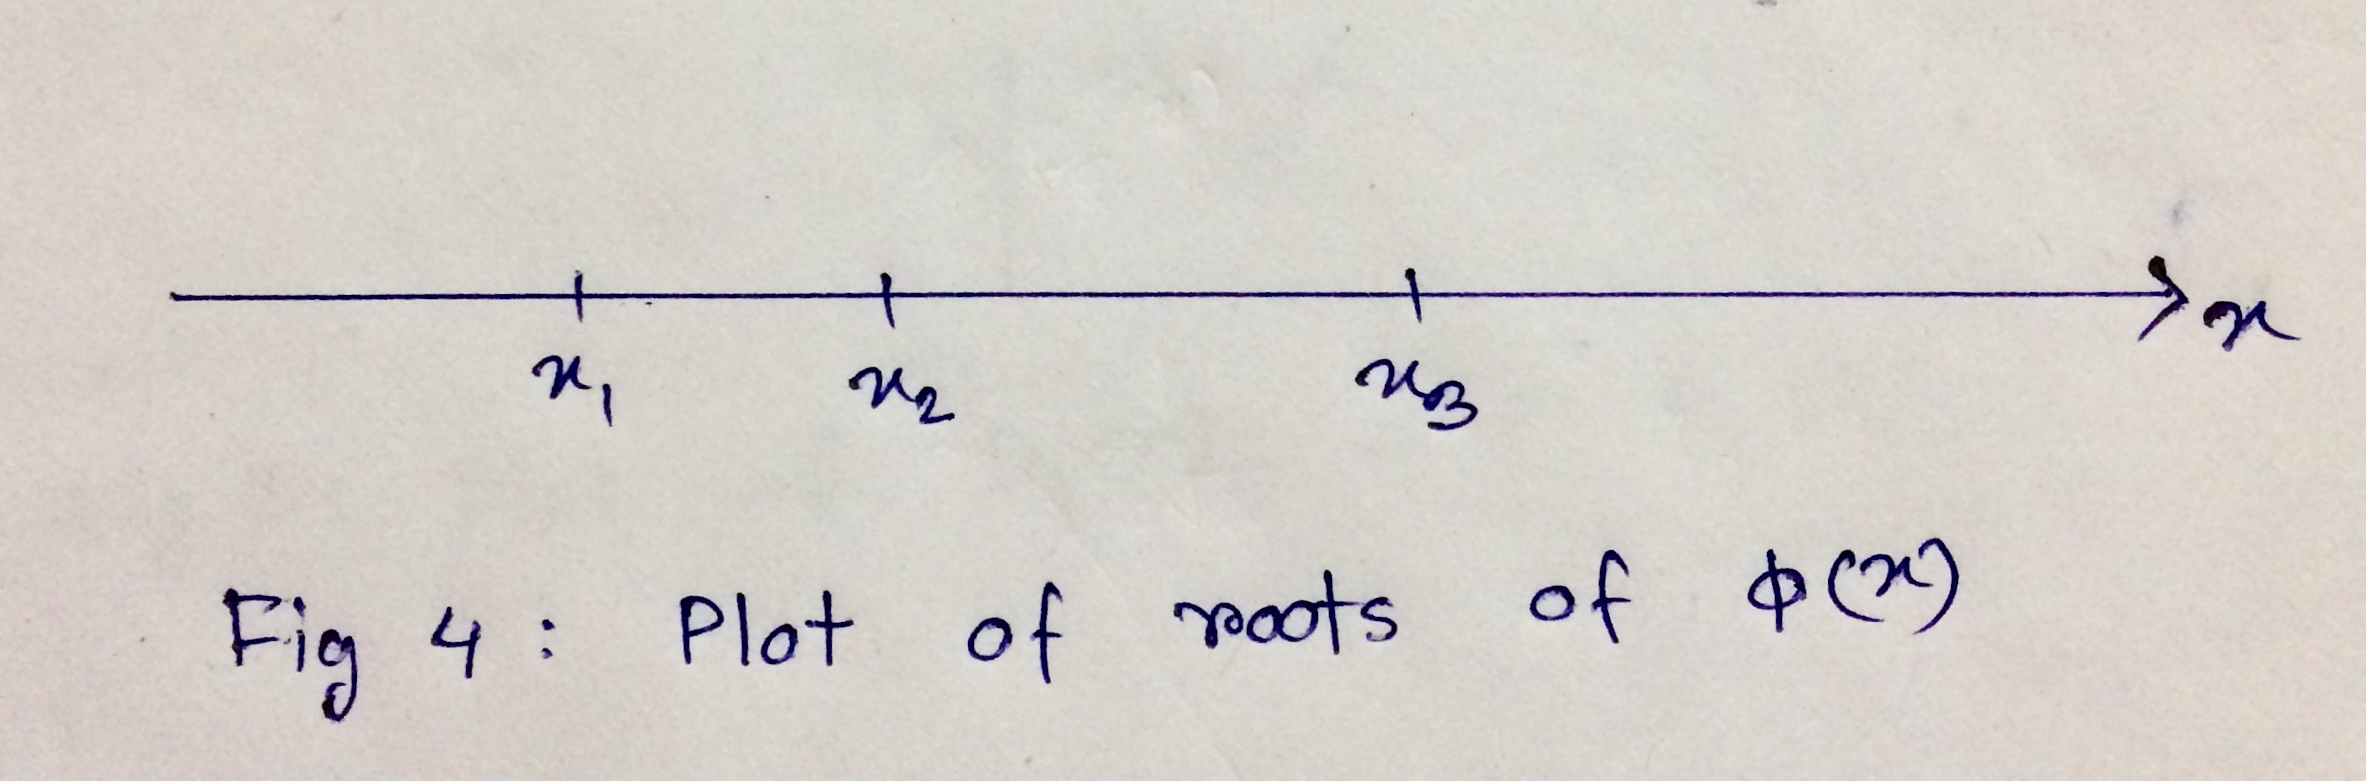
\includegraphics[width=0.6\textwidth]{DiracDeltaFig4.jpg}
\end{center}
In the neighbourhood of any one of the simple roots $x_i$, we can write $$\phi (x) = (x-x_i) \psi(x)$$ where $\psi(x_i) \neq 0$. We have $\psi (x_i) = \left. \frac{\partial \phi(x)}{\partial x} \right|_{x=x_i}$
Now consider the integral
\begin{align*}
&\ \  \int_{-\infty}^{\infty} \delta(\phi(x)) f(x) dx \\
&=\sum_{i=1}^N \int_{x_i - \epsilon}^{x_i + \epsilon} \delta[(x-x_i) \psi(x_i)] f(x) dx \\
&=\sum_{i=1}^N \frac{1}{|\psi(x_i)|} \int_{x_i - \epsilon}^{x_i + \epsilon} \delta(x-x_i) f(x) dx \\
&=\sum_{i=1}^N \frac{1}{|\frac{\partial \phi}{\partial x}|_{x=x_i}} \int_{-\infty}^{\infty} \delta(x-x_i) f(x) dx \\
&=\sum_{i=1}^N \frac{1}{|\frac{\partial \phi}{\partial x}|_{x=x_i}} f(x_i) \\
\end{align*}
The above result is obtained, if we write $$\delta (\phi (x)) = \sum_{i=1}^N \frac{\delta(x-x_i)}{\left| \frac{\partial \phi}{\partial x} \right|_{x=x_i}} $$

\textbf{5.} A frequently used example of the above result is $$\delta (x^2 - a^2) = \frac{1}{2a} \delta(x-a) + \frac{1}{2a} \delta(x+a) \ \ \ \ with a>0$$
Here $$\phi (x) = x^2 - a^2 = (x+a)(x-a)$$.
The two simple roots of $\phi(x)$ are at $x=a$ and $x=-a$. Now, $$\left| \frac{\partial \phi}{\partial x} \right|_{x=a} = |2x|_{x=a} = 2a$$ And $$\left| \frac{\partial \phi}{\partial x} \right|_{x=-a} = |2x|_{x=-a} =|-2a|= 2a$$ So, the above result follows.

\textbf{6.} $$f(x) \delta (x-a) = f(a) \delta(x-a)$$

\textbf{7.} $$\int_{-\infty}^{\infty} \delta (x-y) \delta (y-a) dy = \delta (x-a)$$

\underline{Note 1}:
We have the identity $$x \delta(x) = 0$$. The converse is also true and itcan be shown that the equation $$x u(x) = 0$$ has the general solution $$u(x) = c \delta (x)$$

\underline{Note 2}:
We will now prove an identity which is particularly useful in quantum mechanics. $$\lim_{\epsilon \to 0^+} \int_{-\infty}^{\infty} \frac{1}{x \pm i\epsilon} f(x) dx = P \int_{-\infty}^{\infty} \frac{dx}{x} f(x) \mp i\pi f(0)$$
Or in short $$\lim_{\epsilon \to 0^+} \frac{1}{x \pm i\epsilon} = P\left( \frac{1}{x} \right) \mp i \pi \delta (x)$$
where it is understood that the econd of these two equations have meaning only within an integral. The symbol $P$ means principle part of an integral where the integral has a simple pole. The principle part is defined as $$P \int_A^B \frac{dx}{x} f(x)  = \lim_{n \to 0^+} \left[ \int_A^\eta + \int_\eta^B \right] \frac{dx}{x} f(x)$$

\underline{Proof:}
\begin{equation}
\frac{1}{x \pm i\epsilon} = \frac{x \mp i\epsilon}{x^2+\epsilon^2} = \frac{x}{x^2+\epsilon^2} \mp \frac{i\epsilon}{x^2 + \epsilon^2}
\end{equation}
Now we have $$\lim_{\epsilon \to 0^+} \frac{1}{\pi} \frac{\epsilon}{x^2+\epsilon^2} = \delta(x)$$
So, 
\begin{equation}
\lim_{\epsilon \to 0^+} (\mp)i  \frac{\epsilon}{x^2+\epsilon^2} = \mp i\pi \delta(x)
\end{equation}
Now consider the first term on the right hand side of eqn(11). We multiply this term by a function $f(x)$ which is regular at the origin and then integrate over x. We get,
\begin{equation}
\lim_{\epsilon \to 0^+} \int_{-\infty}^{\infty} \frac{x f(x)}{x^2 + \epsilon^2} dx = \lim_{\epsilon \to 0^+} \left[ \lim_{\eta \to 0^+} \int_{-\infty}^{-\eta} \frac{xf(x)dx}{x^2+\epsilon^2} + \int_{-\eta}^{\eta} \frac{xf(x)dx}{x^2+\epsilon^2} + \int_{\eta}^{\infty} \frac{xf(x)dx}{x^2+\epsilon^2} \right]
\end{equation}
Note that we take the limit over $\eta$ first and then we take the limit over $\epsilon$. Consider now the second integral above $$\lim_{\eta \to 0^+ } \int_{-\eta}^{+\eta} \frac{xf(x)dx}{x^2 + \epsilon^2} = f(0) \lim_{\eta \to 0^+} \frac{1}{2} [ln(x^2+\epsilon^2)]_{x=-\eta}^{x=\eta} = 0$$
If we now reverse the order of the evaluation of limits in eqn (13), the $\epsilon \to 0$ limit causes no difficulties in the other two integrals. We thus have
\begin{align*}
\lim_{\epsilon \to 0^+} \int_{-\infty}^{\infty} \frac{xf(x)dx}{x^2 + \epsilon^2} & = \lim_{\eta \to 0^+} \lim_{\epsilon \to 0^+} \left[ \int_{-\infty}^{-\eta} + \int_{\eta}^{\infty} \right] \frac{xf(x)dx}{x^2 + \epsilon^2} \\
&= \lim_{\eta \to 0^+} \left[ \int_{-\infty}^{-\eta} + \int_{\eta}^{\infty} \right] \frac{dx}{x} f(x) \\
&= P \int_{-\infty}^{\infty} \frac{1}{x} f(x) dx
\end{align*}
This establishes the identity.

\section*{Derivatives Of The Delta Function}
One may define the derivative $\delta^\prime (x)$ of the delta function. When $\epsilon$ is small, the derivative of $D_\epsilon (x)$ has two peaks close to the origin, one peak positive and the other negative as drawn in the figure below.
\vspace{0.2cm}
\begin{center}
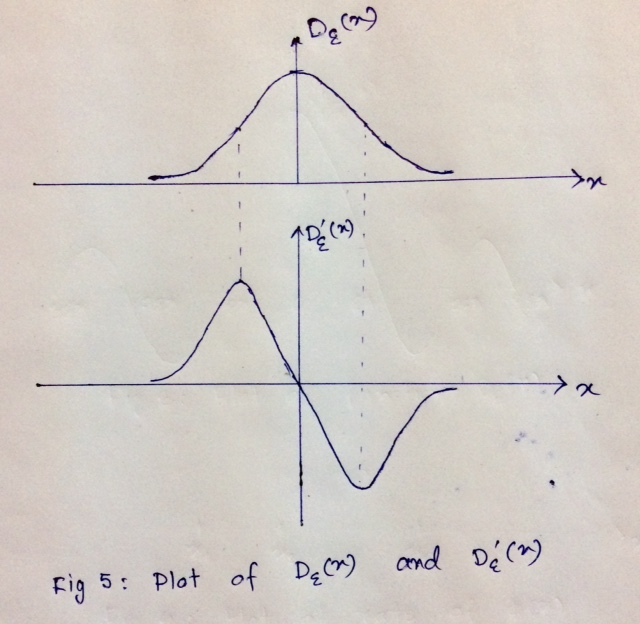
\includegraphics[width=0.8\textwidth]{DiracDeltaFig5.jpg}
\end{center}
As $\epsilon \to 0$, each of these peaks becomes very narrow and very tall, and two peaks each approach very close to the origin. Now, an integration by parts gives
\begin{equation}
\int_{-\infty}^{\infty} dx D_\epsilon^\prime (x) f(x) = [D_\epsilon (x) f(x)]_{-\infty}^{\infty} - \int_{-\infty}^{\infty} dx D_\epsilon (x) f^\prime (x)
\end{equation}
Because $D_\epsilon (x)$ tends to zero as $x \to \pm \infty$, the first term on the right hand side vanishes unless f(x) explodes violently at infinity. So by letting $\epsilon \to 0$, we arrive at the definition of $\delta^\prime (x)$: 
\begin{equation}
\int_{-\infty}^{\infty} \delta^\prime (x) f(x) dx = - \int_{-\infty}^{\infty} \delta (x) f^\prime(x) dx = - f^\prime (0)
\end{equation}
From this, we immediately get 
\begin{equation}
x\delta^\prime (x) = - \delta (x)
\end{equation}
Conversely, it can be shown that the general solution of the equation $$xu(x)=\delta(x)$$ can be written as $$u(x) = - \delta^\prime (x) + c \delta(x)$$ where the second term arises from the homogeneous equation $$x\delta(x)=0$$
From eqn(15) it also follows that
\begin{equation}
\delta^\prime(-x) = - \delta^\prime(x)
\end{equation}
The n-th order derivative of $\delta(x)$ can be defined in the same way. We find
\begin{equation}
\int_{-\infty}^{\infty} \delta^{(n)} (x) f(x) dx = (-1)^n f(0)
\end{equation}
We can prove following properties:

1.$$\delta^{(m)} (x) = (-1)^m \delta^{(m)} (-x)$$

2.$$x^{m+1} \delta^{(m)} (x) = 0$$

3.$$x \delta^{(m)} (x) = -m \delta^{(m-1)} (x)$$

\section*{Integration Of The Delta Function}
Comsider the indefinite integral
\begin{equation}
\theta_\epsilon (x) = \int_{-\infty}^{x} D_\epsilon (y) dy
\end{equation}
A graph of $\theta_\epsilon (x)$ vs x is shown below:
\vspace{0.2cm}
\begin{center}
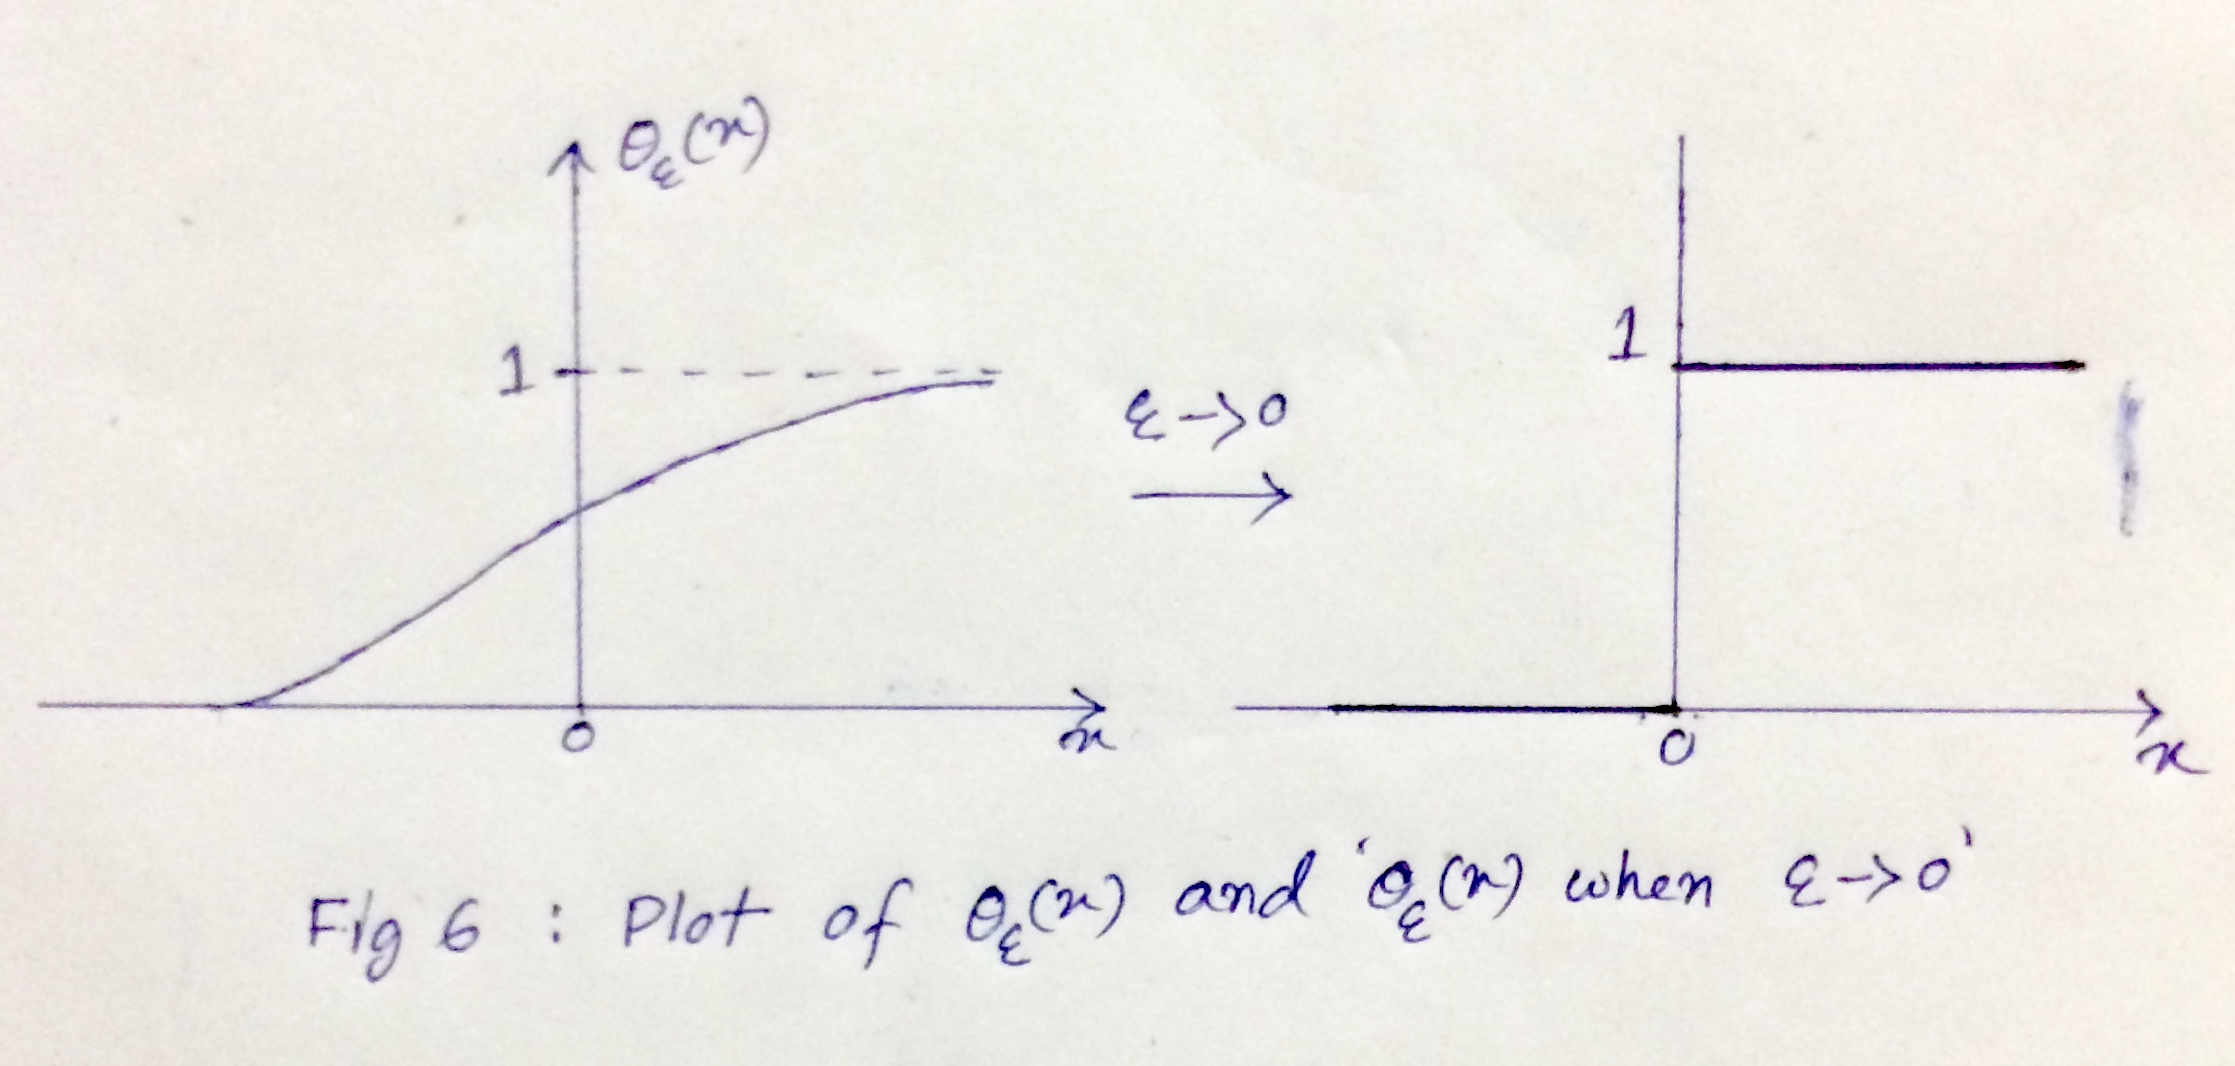
\includegraphics[width=0.8\textwidth]{DiracDeltaFig6.jpg}
\end{center}
As $\epsilon \to 0$, the step in the function $\theta_\epsilon (x)$ gets progressively steeper, until, finally, the function changes abruptly from 0 to 1 at x=0.
Thus, taking the limit $\epsilon \to 0$ in eqn(19), we have
\begin{equation}
\theta (x) = \int_{-\infty}^{x} \delta (x) dx
\end{equation}
where 
\begin{align*}
\theta (x) &= 1 \ \ \ for \ x>0\\
&=0 \ \ \ for \ x<0
\end{align*}
If we differentiate eqn(20) with respect to x, we get 
\begin{equation}
\frac{d\theta (x)}{dx} = \delta (x)
\end{equation}

\section*{Three Dimesional Delta Function}
We define $$\delta (\vec{r}) \equiv \delta (x) \delta (y) \delta (z)$$
In other words, $\delta (\vec{r})$ is zero if any of the coordinates x,y and z is not equal to zero and $\delta (\vec{r})$ tends to infinitely at the origin, i.e, when x=0, y=0 and z=0, such that $$\int_{volume} \delta (\vec{r}) d^3r = 1$$ if the volume of integration contains the origin. We also have $$\int_{volume} \delta (\vec{r}) f(\vec{r}) d^3r = f(0)$$ where again, the volume of integration contains the origin.

Note:

1. $$\delta (\vec{r} - \vec{r}^\prime) = \delta (x-x^\prime) \delta (y-y^\prime) \delta (z-z^\prime)$$

2.$$\delta (\vec{r} - \vec{r}^\prime) d^3r = 1$$ where the volume of integration includes the point $\vec{r}^\prime$, otherwise the integral is zero.

3.$$\int_{volume} \delta (\vec{r} - \vec{r}^\prime) f(\vec{r}) d^3r = f(\vec{r}^\prime)$$ if volume of integration includes the point $\vec{r}^\prime$

\section*{A Useful Formula}
Consider the integral 
\begin{align*}
\int_{-\infty}^{\infty} e^{ikx} dx &= \lim_{L \to \infty} \int_{-L}^{L} e^{ikx}dx \\
&= \lim_{L \to \infty} \frac{1}{ik} \left( e^{ikL} - e^{-ikL} \right) \\
&= \lim_{L \to \infty} \frac{2}{k} \left( \frac{e^{ikL} - e^{-ikL}}{2i} \right) \\
&= \lim_{L \to \infty} \frac{2}{k} \sin kL \\
&= 2\pi \lim_{L \to \infty} \frac{\sin kL}{\pi k} \\
&= 2\pi \delta (k) \\
\end{align*}
Since
\begin{align*}
& \lim_{\epsilon \to 0} \frac{\sin (x/\epsilon)}{\pi x} = \delta (x). \\
& Let, \ \epsilon = \frac{1}{L} \\
& So, \ when, \ L \to \infty, \ then \ \epsilon \to 0. \\
& therefore, \ \lim_{L \to \infty} \frac{\sin kL}{\pi k} = \lim_{\epsilon \to 0} \frac{\sin (k/\epsilon)}{\pi k} 
\end{align*}

Thus
\begin{equation}
\int_{-\infty}^{\infty} e^{ikx} dx = 2\pi \delta (k) 
\end{equation}

In eqn(22) if we integrated with respect to k, we would have $\delta (x)$ on the right handside
\begin{equation}
\int_{-\infty}^{\infty} e^{ikx} dk = 2\pi \delta (x) 
\end{equation}
Also note that in eqn(22) we are integrating over x over its full range of values. Making a change of variable $x \to -x$ does not change the value of the integral. Here we also have 
\begin{equation}
\int_{-\infty}^{\infty} e^{-ikx} dx = 2\pi \delta (k) 
\end{equation}
Similarly in eqn(23), making the change of variable $k \to -k$, doesn't change the value of the integral. So we could also with 
\begin{equation}
\int_{-\infty}^{\infty} e^{-ikx} dk = 2\pi \delta (x) 
\end{equation}
Thus in summery,
\begin{align*}
\int_{-\infty}^{\infty} e^{\pm ikx} dx = 2\pi \delta (k) 
\end{align*}
\begin{align*}
\int_{-\infty}^{\infty} e^{\pm ikx} dk = 2\pi \delta (x) 
\end{align*}
In three dimension
\begin{align*}
\int_{all \ space} e^{\pm i \vec{k}.\vec{r}} d^3r = (2\pi)^3 \delta (\vec{k}) 
\end{align*}
\begin{align*}
\int_{all \ space} e^{\pm i (\vec{k} - \vec{k}^\prime).\vec{r}} d^3r = (2\pi)^3 \delta (\vec{k} - \vec{k}^\prime) 
\end{align*}
\begin{align*}
\int_{all \ space} e^{\pm i \vec{k}.(\vec{r} - \vec{r}^\prime)} d^3k = (2\pi)^3 \delta (\vec{r} - \vec{r}^\prime) 
\end{align*}

\section*{Fourier Transform}
We can always express a function f(x) in the form 
\begin{equation}
f(x) = \int_{-\infty}^{\infty} e^{ikx} \tilde{f}(k) dk
\end{equation}
where $\tilde{f}(k)$ is a function of k, called the fourier transform of f(x). From eqn(26) we can write 
\begin{align*}
\int_{-\infty}^{\infty} e^{-ik^\prime x} f(x) dx &= \int_{-\infty}^{\infty} \int_{-\infty}^{\infty} e^{i(k-k^\prime) x} \tilde{f}(k) dk dx \\
&= (2\pi) \int_{-\infty}^{\infty} \delta(k - k^\prime) \tilde{f}(k) dk \\
&= (2\pi) \tilde{f}(k^\prime) 
\end{align*}
Thus,
\begin{equation}
\tilde{f}(k) = \frac{1}{2 \pi} \int_{-\infty}^{\infty} e^{-ikx} f(x) dx
\end{equation}
The function f(x) and $\tilde{f} (k)$ are Fourier transform of each other. We can write eqn(26) and eqn(27) in a more symmetrical fashion as follows
\begin{equation}
f(x)= \frac{1}{\sqrt{2 \pi}} \int_{-\infty}^{\infty} e^{ikx} \tilde{f}(k) dk
\end{equation}
\begin{equation}
\tilde{f}(k) = \frac{1}{\sqrt{2 \pi}} \int_{-\infty}^{\infty} e^{-ikx} f(x) dx
\end{equation}
In three dimension, we can write
\begin{equation}
f(\vec{r})= \frac{1}{(2 \pi)^{3/2}} \int_{all\ k \ space}  e^{i \vec{k}.\vec{r}} \tilde{f}(\vec{k}) d^3k
\end{equation}
Multiplying this equation by $e^{-i \vec{k}.\vec{r}}$ and integrating over $\vec{r}$, we have
\begin{align*}
\int_{all\ space}  e^{-i \vec{k}^\prime.\vec{r}} f(\vec{r}) d^3r &= \frac{1}{(2 \pi)^{3/2}} \int d^3r \int d^3k e^{i(\vec{k} - \vec{k}^\prime).\vec{r}} \tilde{f}(\vec{k}) \\
&= \frac{1}{(2 \pi)^{3/2}} \int d^3k (2 \pi)^3 \delta (\vec{k} - \vec{k}^\prime) \tilde{f}(\vec{k}) \\
&= (2 \pi)^{3/2} \tilde{f}(\vec{k}^\prime)
\end{align*}
Therefore,
\begin{align*}
\tilde{f}(\vec{k}) = \frac{1}{(2 \pi)^{3/2}} \int e^{-i \vec{k}.\vec{r}} f(\vec{r}) d^3r  
\end{align*}
Thus, if we write
\begin{align*}
f(\vec{r}) = \frac{1}{(2 \pi)^{3/2}} \int e^{i \vec{k}.\vec{r}} \tilde{f}(\vec{k}) d^3k 
\end{align*}
then
\begin{align*}
\tilde{f}(\vec{k}) = \frac{1}{(2 \pi)^{3/2}} \int e^{-i \vec{k}.\vec{r}} \tilde{f}(\vec{r}) d^3r 
\end{align*}

\section*{Parseval Identity}
We can now prove the important identity
\begin{align*}
\int |f(\vec{r})|^2 d^3r = \int |\tilde{f}(\vec{k})|^2 d^3k
\end{align*}
\underline{PROOF:}
\begin{align*}
\int |f(\vec{r})|^2 d^3r &= \int f(\vec{r}) f^*(\vec{r}) d^3r \\
&= \int d^3r \ .\ \frac{1}{(2\pi)^{3/2}} \int e^{i \vec{k}.\vec{r}} \tilde{f} (\vec{k}) d^3k \ .\ \frac{1}{(2\pi)^{3/2}} \int e^{-i \vec{k}^\prime.\vec{r}} \tilde{f}^* (\vec{k}^\prime) d^3k^\prime \\
&= \frac{1}{(2\pi)^3} \int d^3k d^3k^\prime \tilde{f} (\vec{k}) \tilde{f}^* (\vec{k}^\prime) \int d^3r e^{i (\vec{k} - \vec{k}^\prime) . \vec{r}} (2\pi)^3 \delta (\vec{k} - \vec{k}^\prime) \\
&= \int d^3k d^3k^\prime \tilde{f} (\vec{k}) \tilde{f}^* (\vec{k}^\prime) \delta (\vec{k} - \vec{k}^\prime) \\
&= \int d^3k \tilde{f} (\vec{k}) \tilde{f}^* (\vec{k}) \\
&= \int |\tilde{f} (\vec{k})|^2  d^3k  \\
\end{align*}





%
%	Consider the function $D_\epsilon(x)$ given by
%	\begin{eqnarray}
%	D_\epsilon(x) &= 
%		\begin{cases}
%			\frac{1}{\epsilon} \ \ &\text{for} \ \  -\frac{\epsilon}{2} \leq x \leq \frac{\epsilon}{2} \\
%			0 \ \ &\text{for} \ \  |x| > \frac{\epsilon}{2} 
%		\end{cases}
%	\end{eqnarray}
%	where $\epsilon$ is a positive parameter. The plot of the function is shown in figure (\ref{fig.cpt1.figure1}).
%	
%	\begin{figure}
%		\centering
%		\subfloat[]{\includegraphics[width=5cm]{delta.pdf}}
%		\caption{Dirac Delta Function}
%		\label{fig.cpt1.figure1}
%	\end{figure}
%	
%	The integral of the function with respect to $x$ is $1$, i.e.,
%	\begin{equation}
%		\int_{-\infty}^{\infty} D_\epsilon(x) dx = 1
%	\end{equation}
%	Now imagine making $\epsilon$ smaller. As we decrease $\epsilon$, the function gets narrower and taller, but the integral of the function(i.e., the area under graph remains constant at the value $1$).
%	In the limit $\epsilon \rightarrow 0$, the function $D_\epsilon(x)$ collapses to a single  point $x=0$ and gets infinitely tall. So $\lim\limits_{\epsilon \rightarrow \epsilon} D_\epsilon(x)$ is not a function at all and the procedure of taking the limit is not justified.
%	\\
%	
%	However, we can make the limiting procedure meaningful if multiply $D_\epsilon(x)$ by some well defined function $f(x)$, integrate over $x$ and then take the limit $\epsilon \rightarrow 0 $. consider the integral
%	\begin{equation}
%		\int_{-\infty}^{\infty} D_\epsilon(x) f(x) dx
%	\end{equation}
%	where $f(x)$ is a well-defined function. If $\epsilon$ is significantly small, the variation of $f(x)$ over the effective integration interval $[-\epsilon / 2, \epsilon / 2]$ is negligible and $f(x)$ remains practically equal to $f(0)$, therefore,
%	\begin{equation}
%		\int_{-\infty}^{\infty} D_\epsilon (x) f(x) dx \simeq f(0) \int_{-\infty}^{\infty} D_\epsilon (x) dx = f(0)
%	\end{equation}
%	The smaller the value of $\epsilon$, the better the approximation. In the limit $\epsilon \rightarrow 0$, the above equation is exact
%	\begin{equation}
%		\lim\limits_{\epsilon \rightarrow 0}\int_{-\infty}^{\infty} D_\epsilon (x) f(x) dx  = f(0)
%	\end{equation}
%	Now, we define the delta function by the relation
%	\begin{equation}
%		\int_{-\infty}^{\infty} \delta(x) f(x) dx \  _=^{def}  \lim\limits_{\epsilon \rightarrow 0}\int_{-\infty}^{\infty} D_\epsilon (x) f(x) dx  = f(0)
%	\end{equation}
%	This equation is valid for any function $f(x)$ defined at the origin. More generally, $\delta(x - x_0)$ is defined as,
%	\begin{equation}
%		\int_{-\infty}^{\infty} \delta(x - x_0) f(x) dx \ = f(x_0)
%	\end{equation}
%	Actually, the integral notation $\int_{-\infty}^{\infty} \delta(x) f(x) dx$ is not justified because $\delta(x)$ is not really a function. Physically, there is no problem since it becomes impossible to distinguish between $D_\epsilon(x)$ and $\delta(x)$ as soon as $\epsilon$ becomes negligible compared to all distances involved in a physical problem. Whenever a mathematical difficulty might arise, all we need to do is to assume that $\delta(x)$ is actually $D_\epsilon(x)$ with $\epsilon$ extremely small but not strictly zero.
%	\\
%	Formally, we can express $\delta(x)$ as a limit of a square of proper functions : 
%	\begin{equation}
%		\lim\limits_{\epsilon \rightarrow 0} D_\epsilon(x) \equiv \delta(x)
%	\end{equation}
%	Here $D_\epsilon(x)$, which is a proper function of $x$ is called the representation of the delta function. One representation is the "square function" given at the beginning. The representation is not unique. There are other functions which approach the delta function when appropriate limits are taken.
%	
%	\section{Other representation of delta function}
%		\begin{enumerate}
%			\item 
%			Consider the function
%			\begin{equation}
%				D_\epsilon(x) = \frac{1}{\epsilon \sqrt{\pi}} e^{-x^2/\epsilon^2}  \ \ \ (\epsilon > 0)
%				\label{eqn.other-reps-exp}
%			\end{equation}
%			For each value of the parameter $\epsilon$, this function satisfies
%			\begin{equation}
%			\int_{-\infty}^{\infty} D_\epsilon(x) dx = 1
%			\end{equation}
%		
%		\begin{figure}
%			\centering
%			\subfloat[]{\includegraphics[width=5cm]{chapter1-delta-reps-exp.pdf}}
%			\subfloat[]{\includegraphics[width=5cm]{chapter1-delta-reps-sine.pdf}}
%			\caption{Plot of function $D_\epsilon(x)$ for (a) equation (\ref{eqn.other-reps-exp}) (b) and equation (\ref{eqn.other-reps-sin})}
%			\label{fig.cpt1.figure2}
%		\end{figure}
%		
%		
%		When plotted against $x$, the function has a peak at the origin. The peak has a height of $\frac{1}{\epsilon \sqrt{\pi}}$ and a width of order $\epsilon$ (exactly how the width is defined doesn't matter). So if $\epsilon$ is allowed to become very small, the peak becomes very tall and very narrow. Outside the peak the function becomes extremely small. Thus we have
%		\begin{equation}
%		\delta(x) = \lim\limits_{\epsilon \rightarrow 0}\frac{1}{\epsilon \sqrt{\pi}} e^{-x^2/\epsilon^2}
%		\end{equation}
%		
%		%% proof
%		
%		\item
%		Consider another function
%		\begin{equation}
%			D_\epsilon(x) = \frac{1}{\pi} \frac{\sin(x/\epsilon)}{x} \ \ \ \ (\epsilon > 0)
%			\label{eqn.other-reps-sin}
%		\end{equation} 
%		
%
%		
%		For any value of the parameter $\epsilon$ we have 
%		\begin{equation}
%			\int_{-\infty}^{\infty} D_\epsilon(x) dx = 1
%		\end{equation}
%		A plot of the function $D_\epsilon(x)$ shows that it has the value $\frac{1}{\epsilon \pi}$ at $x=0$ and it oscillates with decreasing amplitude as $|x|$ increases. The width of the central maxima is of the order of $\epsilon$ and the period of oscillation with respect to $x$ is $2 \pi \epsilon$.\\
%		Thus the limit of this function as $\epsilon \rightarrow 0 $ has all the properties of the delta function : it becomes infinitely large at $x=0$, it has unit integral, and infinitely rapid oscillations as $|x|$ increases means that the entire contribution to an integral containing this function comes from an infinitesimal neighborhood of $x=0$.\\
%		We can therefore write,
%		\begin{equation}
%			\delta(x) = \lim\limits_{\epsilon \rightarrow 0} \frac{1}{\pi} \frac{\sin(x/\epsilon)}{x}
%		\end{equation}
%
%		\item
%		We can also show that
%		\begin{eqnarray}
%			\delta(x) &= \lim\limits_{\epsilon \rightarrow 0} \frac{1}{2\epsilon} e^{-|x| / \epsilon} \\
%			\delta(x) &= \lim\limits_{\epsilon \rightarrow 0} \frac{1}{\pi} \frac{\epsilon}{x^2 + \epsilon^2} \\
%			\delta(x) &= \lim\limits_{\epsilon \rightarrow 0} \frac{\epsilon}{\pi} \frac{\sin^2(x/\epsilon)}{x^2}
%		\end{eqnarray}
%		
%		\end{enumerate}	
%	\section{Properties of the delta function}
%		It is important to note that, because of its singular $@@@@@@$ , the $\delta$ function cannot be the end result of a calculation, and has meaning only so long as a subsequent integral over its argument is carried out. With this understanding we can write down some relations between delta functions.
%		\begin{enumerate}[label=\textbf{Property \ \arabic*},start=1]
%			\item 
%			The delta function is a even function
%			\begin{equation}
%				\delta(-x) = \delta(x)
%			\end{equation}
%			
%			\item
%			\begin{equation}
%				x \delta(x) = 0
%			\end{equation}
%			
%			\item
%			\begin{equation}
%			\delta(a x) = \frac{1}{|a|} \delta(x)
%			\end{equation}
%			proof: Consider the integral
%			\begin{equation}
%				I = \int_{-\infty}^{\infty} \delta(a x) f(x) dx
%			\end{equation}
%			Since the delta function is even in its argument, it doesn't matter if we replace $a$ by $|a|$ in the argument. Thus
%			\begin{equation}
%				I = \int_{-\infty}^{\infty} \delta(|a| x) f(x) dx
%			\end{equation}
%			Making the change in variable $ y = |a| x$ we have,
%			\begin{eqnarray}
%				I &= \frac{1}{|a|}\int_{-\infty}^{\infty} \delta(y) f(y/|a|) dx \nonumber \\
%				&= \frac{1}{|a|} f(0) \nonumber
%			\end{eqnarray}			
%			or
%			\begin{equation}
%				\int_{-\infty}^{\infty} \delta(a x) f(x) dx = \frac{1}{|a|} \int_{-\infty}^{\infty} \delta(x) f(x) dx
%			\end{equation}
%			or
%			\begin{equation}
%				\delta(a x) = \frac{1}{|a|} \delta(x)
%			\end{equation}
%			
%			
%			\item
%			More generally
%			\begin{equation}
%				\delta(\phi(x)) = \sum_{i} \frac{\delta(x - x_i)}{\left|\frac{\partial\phi}{\partial x}\right|_{x_i}}
%			\end{equation}
%			where the sum sums over the $x_i$'s which are simple roots of $\phi(x)$.
%			
%			proof : let $x_1 , x_2, \ldots , x_N$ be the simple roots of $\phi(x)$,
%			
%			%figure
%			
%			In the neighborhood of any one of the simple roots $x_i$, we can write
%			@@@@@@@
%			\begin{equation}
%				\phi(x) = (x - x_i) \psi(x)
%			\end{equation}
%			or ???????
%			\begin{equation}
%				\phi(x) = (x - x_i) \psi(x_i)
%			\end{equation}
%			
%			where $\psi(x_i) \neq 0$. We have
%			\begin{equation}
%				\psi(x_i) = \left|\frac{\partial \phi(x)}{\partial x} \right|_{x=x_i}
%			\end{equation}
%			Now, consider the integral
%			\begin{eqnarray}
%				I &= \int_{-\infty}^{\infty} \delta(\phi(x)) f(x) dx  \nonumber \\
%				&= \sum_{i=1}^{N} \int_{x_i - \epsilon}^{x_i + \epsilon} \delta[(x-x_i) \psi(x_i)] f(x) dx \nonumber \\
%				&= \sum_{i=1}^{N} \frac{1}{|\psi(x_i)|}\int_{x_i - \epsilon}^{x_i + \epsilon} \delta(x-x_i) f(x) dx \nonumber \\
%				&= \sum_{i=1}^{N} \frac{1}{ \left|\frac{\partial \phi(x)}{\partial x} \right|_{x=x_i}}\int_{-\infty}^{\infty} \delta(x-x_i) f(x) dx \nonumber \\
%				&= \sum_{i=1}^{N} \frac{1}{ \left|\frac{\partial \phi}{\partial x} \right|_{x=x_i}} f(x_i) \nonumber
%			\end{eqnarray}
%			The above result is obtained if we write
%			\begin{equation}
%				\delta(\phi(x)) = \sum_{i=1}^{N} \frac{\delta(x - x_i)}{\left|\frac{\partial \phi}{\partial x}\right|_{x=x_i}}
%			\end{equation}
%			
%			
%			\item
%			A frequently used example of the above result is
%			\begin{equation}
%				\delta(x^2 - a^2) = \frac{1}{2 a} \delta(x - a) + \frac{1}{2 a} \delta(x + a) \ \ \ \ (a > 0)
%			\end{equation}
%			
%			Here
%			\begin{equation}
%				\phi(x) = x^2 - a^2 = (x-a)(x+a)
%			\end{equation}
%				The two simple roots of $\phi(x)$ are at $x=a $ and $x=-a$. Now
%				\begin{eqnarray}
%					\left|\frac{\partial \phi}{\partial x}\right|_{x=a} = \left|2 x\right|_{x=a} = 2a  \\
%					\left|\frac{\partial \phi}{\partial x}\right|_{x=a} = \left|-2 x\right|_{x=-a} = 2a 
%				\end{eqnarray}
%				$\therefore$ The above result follows.
%				
%				\item
%				\begin{equation}
%					f(x) \delta(x-a) = f(a) \delta(x-a)
%				\end{equation}
%
%				\item
%				\begin{equation}
%					\int \delta(x-y) \delta(y-a) dy = \delta(x-a)
%				\end{equation}
%				
%			
%		\end{enumerate}
%		
%		\subsection{Notes}
%		\begin{enumerate}[label=\textbf{Note : \ \arabic*},start=1]
%			\item 
%			We have the identity
%			\begin{equation}
%				x\delta(x) = 0
%			\end{equation}
%			The converse is also true and it can be shown that the equation
%			\begin{equation}
%				x u(x) = 0
%			\end{equation}
%			has the general solution
%			\begin{equation}
%				u(x) = c \delta(x)
%			\end{equation}
%			
%			
%			\item
%			We will now prove an identity which is particularly useful in Quantum Mechanics.
%			\begin{equation}
%				\lim\limits_{\epsilon \rightarrow 0^+} \int_{-\infty}^{\infty} \frac{1}{x \pm \imath \epsilon} f(x) dx = \rho \int_{-\infty}^{\infty} \frac{dx}{x}f(x) \mp \imath\pi f(0)
%			\end{equation}
%			or in short
%			\begin{equation}
%				\lim\limits_{\epsilon \rightarrow 0^+} \frac{1}{x \pm \imath \epsilon} = \rho(\frac{1}{x}) \mp \imath \pi \delta(x)
%			\end{equation}
%			Where it is understood that the second of these two equations have meaning only within an integral.\\
%			The symbol $\rho$ means principle part of an integral where the integral has a single pole. The principle part is defined as
%			\begin{equation}
%				\rho \int_{-A}^{B} \frac{dx}{x} f(x) dx = \lim\limits_{\eta \rightarrow 0^+} \left[\int_{-A}^{-\eta} + \int_{\eta}^{B}\right] \frac{dx}{x} f(x)
%			\end{equation}
%			\textbf{proof :}
%			\begin{equation}
%				\frac{1}{x \pm \imath \epsilon} = \frac{x \mp \imath\epsilon}{x^2 + \epsilon^2} = \frac{x}{x^2 + \epsilon^2} \mp \frac{\imath \epsilon}{x^2 + \epsilon^2}
%			\end{equation}
%			Now we have
%			\begin{eqnarray}\label{eqn:1}
%				\lim\limits_{\epsilon \rightarrow 0^+} \frac{1}{\pi} \frac{\epsilon}{x^2 + \epsilon^2} &= \delta(x) \nonumber \\
%				\lim\limits_{\epsilon \rightarrow 0^+} (\mp) \imath \frac{\epsilon}{x^2 + \epsilon^2} &= \mp \imath \pi \delta(x)
%			\end{eqnarray}
%			Now consider the first term on the right hand side of equation  \ref{eqn:1}. We multiply this term by a function $f(x)$ which is regular at the origin and then integrate over $x$. We get
%			\begin{equation}\label{eqn:2}
%				\lim\limits_{\epsilon \rightarrow 0^+} \int_{-\infty}^{\infty} \frac{x f(x)}{x^2 + \epsilon^2} dx
%				=\lim\limits_{\epsilon \rightarrow 0^+}\left[
%				\lim\limits_{\eta \rightarrow 0^+}\left[ \int_{-\infty}^{-\eta} \frac{x f(x)}{x^2 + \epsilon^2}
%				+\int_{-\eta}^{\eta} \frac{x f(x)}{x^2 + \epsilon^2}
%				+\int_{\eta}^{\infty} \frac{x f(x)}{x^2 + \epsilon^2} dx\right]\right]
%			\end{equation}
%			Note that we take the limit over $\eta$ first and then we take the limit over $\epsilon$. Consider now the second integral above
%			\begin{equation} 
%				\lim\limits_{\eta \rightarrow 0^+} \int_{-\eta}^{+\eta} \frac{x f(x)}{x^2 + \epsilon^2} = f(0) \lim\limits_{\eta \rightarrow 0^+} \frac{1}{2}  \left[\ln({x^2 + \epsilon^2}
%				)\right]_{x=-\eta}^{x=\eta} = 0
%			\end{equation}
%			If we now reverse the order of the evaluation of limits in equation \ref{eqn:2}, the $\epsilon \rightarrow 0$ limit causes no difficulties in the other two integrals.
%			Thus we have
%			\begin{eqnarray}
%				&\lim\limits_{\epsilon \rightarrow 0^+} \int_{-\infty}^{\infty} \frac{x dx}{x^2 + \epsilon^2} f(x)\nonumber \\
%				 = &\lim\limits_{\eta \rightarrow 0^+} \lim\limits_{\epsilon \rightarrow 0^+} \left[\int_{-\infty}^{-\eta} + \int_{\eta}^{\infty}\right] \frac{x dx}{x^2 + \epsilon^2} f(x) \nonumber \\
%				 = &\lim\limits_{\eta \rightarrow 0^+} \left[\int_{-\infty}^{-\eta} + \int_{\eta}^{\infty}\right] \frac{dx}{x} f(x) \nonumber\\
%				 = & \rho \int_{-\infty}^{\infty} \frac{1}{x} f(x) dx \nonumber
%			\end{eqnarray}
%			This establishes the identity.
%		\end{enumerate}
%		
%	\section{Derivatives of the delta function}
%		One may define the derivative $\delta^\prime(x)$ of the delta function. When $\epsilon$ is small, the derivative of $D_\epsilon(x)$ has two peaks close to the origin, one peak is positive and the other is negative as drawn in the figure below
%		
%		\begin{figure}
%			\centering
%			\subfloat[]{\includegraphics[height=8cm,width=5cm]{chapter1-delta-reps-exp-derivative.pdf}}
%			\caption{(a) Derivative of Delta Function}
%			\label{}
%		\end{figure}
%		% figure
%		
%		
%		As $\epsilon \rightarrow 0$, each of these peaks becomes very narrow and very tall, and two peaks each approach very close to the origin. \\
%		Now the integration by parts gives
%		\begin{equation}
%			\int_{-\infty}^{\infty} dx D_\epsilon^\prime(x) f(x) = \left[D_\epsilon(x) f(x)\right]_{-\infty}^{\infty} - \int_{-\infty}^{\infty} dx D_\epsilon(x) f^\prime(x)
%		\end{equation}
%		Because $D_\epsilon(x)$ tens to zero as $x \rightarrow \pm \infty$, the first term on the right hand side vanishes unless $f(x)$ $@@@@@@@$ violently at infinity. So by letting $\epsilon \rightarrow 0$, we arrive at the definition of $\delta^\prime(x)$
%		\begin{equation}\label{eqn:3}
%			\int_{-\infty}^{\infty} \delta^\prime(x) f(x) dx = - \int_{-\infty}^{\infty} \delta(x) f^\prime(x) dx = - f^\prime(0)
%		\end{equation}
%		From this we immediately get
%		\begin{equation}
%			x \delta^\prime(x) = -\delta(x)
%		\end{equation}
%		Conversely, it can be shown that the general solution of the equation
%		\begin{equation}
%			x u(x) = \delta(x)
%		\end{equation}
%		can be written as
%		\begin{equation}
%			u(x) = -\delta^\prime(x) + c \delta(x)
%		\end{equation}
%		Where the second term arises from the homogeneous equation $x \delta(x) = 0$.
%		From equation  \ref{eqn:3}  it also follows that 
%		\begin{equation}
%			\delta^\prime(-x) = - \delta^\prime(x)
%		\end{equation}
%		The $n^{th}$ order derivative of $\delta(x)$ can be defined in the same way. We find
%		\begin{equation}
%			\int_{-\infty}^{\infty} \delta^{(n)}(x) f(x) dx = (-1)^{n} f(0)
%		\end{equation}
%		We can prove the following properties:
%		\begin{eqnarray}
%			\delta^{(m)}(x) &= (-1)^m \delta^{(m)} (-x) \\
%			x^{m+1} \delta^{(m)}(x) &= 0 \\
%			x\delta^{(m)}(x) &= -m \delta^{(m-1)} (x)
%		\end{eqnarray}
%		
%		
%	\section{Integration of the delta function}
%		Consider the indefinite integral
%		\begin{equation}\label{eqn:4}
%			\Theta_\epsilon(x) = \int_{-\infty}^{x}  D_\epsilon(y) dy
%		\end{equation}
%		A graph of $\Theta_\epsilon(x)$ vs $x$ is shown below
%		
%		%figure
%		
%		As $\epsilon \rightarrow 0$, the step in the function $\Theta_\epsilon(x)$ gets progressively steeper, until, finally, the function changes abruptly from $0$ to $1$ at $x=0$.
%		Thus taking the limit $\epsilon \rightarrow 0$ in equation \ref{eqn:4} we have
%		\begin{equation}\label{eqn:5}
%			\Theta(x) = \int_{-\infty}^{x} \delta(x) dx
%		\end{equation}
%		Where
%		\begin{equation}
%			\Theta(x) = 
%			\begin{cases}
%				1 \ \ \text{for} \ \ x > 0 \\
%				0 \ \ \text{for} \ \ x < 0
%			\end{cases}
%		\end{equation}
%		If we differentiate equation \ref{eqn:5} with respect to $x$,\\
%		we get
%		\begin{equation}
%			\frac{d \Theta(x)}{dx} = \delta(x)
%		\end{equation}
%		
%	\section{Three - dimensional delta function}
%		\begin{equation}
%			\delta(\vec{r}) _=^{def} \delta(x) \delta(y) \delta(z)
%		\end{equation}
%		In other words, $\delta(\vec{r})$ is zero if any of the coordinates $x, y, z$ is not equal to zero and $\delta(\vec{r})$ tends to infinity at the origin, i.e., when $x=0, y=0, z=0$, such that 
%		\begin{equation}
%			\int_{volume} \delta(\vec{r}) d^3 r = 1
%		\end{equation}
%		if the volume of the integration contains the origin. We also have
%		\begin{equation}
%			\int \delta(\vec{r}) f(\vec{r}) d^3 r = f(0)
%		\end{equation}
%		where again the volume of the integration includes the origin.
%		\textbf{Note:}
%		\begin{eqnarray}
%			\delta(\vec{r} - \vec{r^\prime}) &= \delta(x - x^\prime) \delta(y - y^\prime) \delta(z-z^\prime) \\
%			\int_{v}\delta(\vec{r} - \vec{r^\prime}) d^3r &= 1
%		\end{eqnarray}
%		where the volume of integration includes the point $\vec{r}^\prime$. Otherwise the integral is zero.
%		\begin{equation}
%			\int_{v}\delta(\vec{r} - \vec{r^\prime}) f(\vec{r}) d^3r = f(\vec{r^\prime})
%		\end{equation}
%		if V includes the point $\vec{r^\prime}$.
%		
%		\textbf{A useful formula}
%		Consider the integral
%		\begin{eqnarray}
%			\int_{-\infty}^{\infty} e^{\imath k x} dx 
%			&= \lim\limits_{L \rightarrow \infty} \int_{-L}^{L} e^{\imath k x} dx \nonumber \\
%			&= \lim\limits_{L \rightarrow \infty} \frac{1}{\imath k} \left(e^{\imath k L} - e^{-\imath k L}\right) \nonumber \\
%			&= \lim\limits_{L \rightarrow \infty} \frac{2}{k} \left(\frac{e^{\imath k L} - e^{-\imath k L}}{2\imath}\right) \nonumber \\
%			&= \lim\limits_{L \rightarrow \infty} \frac{2}{k} \sin(k L) \nonumber \\
%			&= 2\pi \lim\limits_{L \rightarrow \infty} \frac{\sin(k L
%				)}{\pi k} \nonumber \\
%			&= 2\pi \delta(k)
%		\end{eqnarray}
%		using 
%		\begin{equation}
%			\lim\limits_{\epsilon \rightarrow 0} \frac{\sin(x /\epsilon
%				)}{\pi x} = \delta(x)
%		\end{equation}
%		Thus
%		\begin{equation}\label{eqn:6}
%			\int_{-\infty}^{\infty} e^{\imath k x} dx = 2\pi \delta(k)
%		\end{equation}
%		In equation \ref{eqn:6} if we integrate with respect to $k$, we would have $delta(x)$ on the right hand side,
%	
%	%%%%%%%%%%%%%%%%%%%%%%%%%%%% equation number
%	
%		\begin{equation}\label{eqn:100}
%		\int_{-\infty}^{\infty} e^{\imath k x} dk = 2\pi \delta(x)
%		\end{equation}
%		Also note that in equation \ref{eqn:6} we are integrating over its full range of values. Making a change of variable $x \rightarrow -x$ does not change the value of the integral. Hence we also have
%		
%		\begin{equation}\label{eqn:101}
%		\int_{-\infty}^{\infty} e^{-\imath k x} dx = 2\pi \delta(k)
%		\end{equation}
%		Similarly, in equation \ref{eqn:100} making the change $k \rightarrow -k$, doesn't change the value of the integral. So we could also write
%		\begin{equation}\label{eqn:102}
%		\int_{-\infty}^{\infty} e^{-\imath k x} dk = 2\pi \delta(x)
%		\end{equation}
%		
%		Thus in summary
%		\begin{eqnarray}\label{eqn:103-104}
%			\int_{\pm \infty}^{\infty} e^{-\imath k x} dx &= 2\pi \delta(k)
%			\int_{\pm \infty}^{\infty} e^{-\imath k x} dk &= 2\pi \delta(x)
%		\end{eqnarray}
%		In three dimensions
%		\begin{eqnarray}\label{eqn:105-107}
%			\int_{all\ space} e^{\pm \imath \vec{k} . \vec{r}} d^3\vec{r} &= (2\pi)^3 \delta(\vec{k}) \\
%			\int_{all\ space} e^{\pm \imath (\vec{k} - \vec{k^\prime}) . \vec{r}} d^3\vec{r} &= (2\pi)^3 \delta(\vec{k} - \vec{k^\prime}) \\
%			\int_{all\ space} e^{\pm \imath \vec{k} . (\vec{r} - \vec{r^\prime})} d^3\vec{r} &= (2\pi)^3 \delta(\vec{r} - \vec{r^\prime}) \\
%		\end{eqnarray}
%		
%	\section{Fourier Transformation}
%		We can always express a function $f(x)$ in the form
%		\begin{eqnarray}\label{eqn:108}
%			f(x) = \int_{-\infty}^{\infty} e^{\imath k x} \tilde{f}(k) dk
%		\end{eqnarray}
%		where $\tilde{f}(k)$ is a function of $k$, called the fourier transform of $f(x)$. From eqnarray \ref{eqn:108} we can write
%		
%		\begin{eqnarray}\label{eqn:109}
%			\int_{-\infty}^{\infty} e^{-\imath k^\prime x} f(x) dx 
%			&= \int_{-\infty}^{\infty} \int_{-\infty}^{\infty} e^{i(k-k^\prime) x} \tilde{f}(k) dk dk^\prime \nonumber \\
%			&= 2 \pi \int_{-\infty}^{\infty} \delta(k-k^\prime) \tilde{f}(k) dk \nonumber \\
%			&= 2\pi \tilde{f}(k^\prime) 
%		\end{eqnarray}
%		
%		Thus
%		\begin{eqnarray}\label{eqn:110}
%			\tilde{f}(k) = \frac{1}{2\pi} \int_{-\infty}^{\infty} e^{-\imath k x} f(x) dx
%		\end{eqnarray}
%		Thus functions $f(x)$ and $\tilde{f}(k)$ are Fourier transform of each other. We can write eqnarray \ref{eqn:108} and \ref{eqn:110} in a more symmetrical fashion as follows:
%		\begin{eqnarray}\label{eqn:111}
%		f(x) = \frac{1}{\sqrt{2\pi}} \int_{-\infty}^{\infty} e^{\imath k x} \tilde{f}(k) dk
%		\end{eqnarray}
%		\begin{eqnarray}\label{eqn:112}
%			\tilde{f}(k) = \frac{1}{\sqrt{2\pi}} \int_{-\infty}^{\infty} e^{-\imath k x} f(x) dx
%		\end{eqnarray}
%		In three dimension, we can write
%		\begin{eqnarray}\label{eqn:113}
%			f(\vec{r}) = \frac{1}{(2\pi)^{3/2}} \int_{all\ k-space} e^{i \vec{k} . \vec{r}} \tilde{f}(\vec{k}) d^3k
%		\end{eqnarray}
%		multiplying eqnarray \ref{eqn:113} by $e^{-i\vec{k^\prime} . \vec{r}} $ and integrating over $\vec{r}$, we have
%		\begin{eqnarray}\label{eqn:114}
%			\int_{all\ space} e^{-i\vec{k^\prime} . \vec{r}} f(\vec{r}) d^3 r
%			&= \frac{1}{(2\pi)^{3/2}} \int d^3 r \int d^3 k \ e^{i (\vec{k} - \vec{k^\prime}). \vec{r}} \tilde{f}(\vec{k}) \nonumber \\
%			&= \frac{1}{(2\pi)^{3/2}} \int d^3 k (2\pi)^3 \delta(\vec{k} - \vec{k^\prime}) \tilde{f}(\vec{k}) \nonumber \\
%			&= \frac{1}{(2\pi)^{-3/2}} \tilde{f}(\vec{k^\prime})
%		\end{eqnarray}
%		
%		Therefore
%		\begin{eqnarray}\label{eqn:115}
%			\tilde{f}(\vec{k}) = \frac{1}{(2\pi)^{3/2}} \int e^{-i\vec{k} . \vec{r}} f(\vec{r}) d^3 r
%		\end{eqnarray}
%		Thus we can write 
%		\begin{eqnarray}\label{eqn:116}
%		f(\vec{r}) = \frac{1}{(2\pi)^{3/2}} \int e^{i\vec{k} . \vec{r}} \tilde{f}(\vec{k}) d^3 k
%		\end{eqnarray}
%		\begin{eqnarray}\label{eqn:117}
%		\tilde{f}(\vec{k}) = \frac{1}{(2\pi)^{3/2}} \int e^{-i\vec{k} . \vec{r}} f(\vec{r}) d^3 r
%		\end{eqnarray}
%		
%		\textbf{Parseval's Identity:}\\
%		We can now  prove the important identity
%		\begin{eqnarray}\label{eqn:118}
%			\int |f(\vec{r})|^2 d^3r = \int |\tilde{f}(\vec{k})|^2 d^3k
%		\end{eqnarray}
%		proof:
%		\begin{eqnarray}
%			\int |f(\vec{r})|^2 d^3r
%			&= \int f(\vec{r}) f^*(\vec{r}) d^3r \nonumber \\
%			&= \int d^3r \frac{1}{(2\pi)^{3/2}} \int e^{\imath\vec{k} . \vec{r}} \tilde{f}(\vec{k}) d^3k \frac{1}{(2\pi)^{3/2}} \int e^{-\imath\vec{k^\prime} . \vec{r}} \tilde{f}^*(\vec{k^\prime}) d^3k^\prime \nonumber \\
%			&= \frac{1}{(2\pi)^3} \int d^3k\ d^3k^\prime \tilde{f}(\vec{k}) \tilde{f}^*(\vec{k^\prime}) \int d^3r \ e^{\imath(\vec{k} - \vec{k^\prime}).\vec{r}} \nonumber \\
%			&= \frac{1}{(2\pi)^3} \int d^3k\ d^3k^\prime \tilde{f}(\vec{k}) \tilde{f}^*(\vec{k^\prime}) (2\pi)^3 \delta(\vec{k} - \vec{k^\prime}) \nonumber \\
%			&= \int d^3k\ \tilde{f}(\vec{k}) \tilde{f}^*(\vec{k}) \nonumber \\
%			&= \int |\tilde{f}(\vec{k})|^2 d^3k
%		\end{eqnarray}
%		
%		
%		
%		
%		